\chapter{Digital Model for Elastica}
\label{chapter:digital-model-elastica}

In this chapter we review the elastica energy and some of its properties. Next, we introduce the digital version of the elastica using multigrind convergent estimators of length and curvature. Finally, we describe a theoretical optimization model for the minimization of the digital elastica.

\section{Continuous and Digital Elastica}
	\sketch{To be developed...}
	
	
	Given an Euclidean shape $X$, its digital elastica $\hat{E}$ is defined as
	\begin{align}
	\hat{E}( D_h(X) ) = \sum_{\dot{\vec{e}} \in \partial D_h(X)}{ \hat{s}( \dot{\vec{e}})\left(\; \alpha + \beta \hat{\kappa}_{r}^2(D_h(X),\dot{\vec{e}},h) \; \right)},
	\label{eq:digital-elastica}
	\end{align}
	
where $\dot{\vec{e}}$ denotes the center of the edge $\vec{e}$. In the
expression above, we will substitute an arbitrary subset $Z$ of
$\mathbb{Z}^2$ to $D_h(X)$ since the continuous shape $X$ is unknown.
In the following we omit the grid step $h$ to simplify expressions
(or, putting it differently, we assume that the shape of interest is
rescaled by $1/h$ and we set $h=1$). 

In the next section, we describe a combinatorial scheme that permit us to find the minimum digital shape with respect the digital elastica energy for some neighborhood of shapes of $S$. 

\section{Local Combinatorial Scheme}\label{sec:local-combinatorial-scheme}

Given a digital shape $S^{(0)}$ we describe a process that generates a
sequence $S^{(i)}$ of shapes with non-increasing Elastica energy. The
idea is to define a neighborhood of shapes $\mathcal{N}^{(i)}$ to the
shape $S^{(i)}$ and choose the element of $\mathcal{N}^{(i)}$ with
lowest energy.  The process is suited for the integral invariant
estimator but also for other curvature estimators, for example, MDCA
\cite{roussillon11mdca}. As a matter of fact, our experiments have
shown that either estimators induce similar results.

Let $S$ be a $2$-dimensional digital shape embedded in a domain $\Omega \subset \mathbb{Z}^2$. We adopt the cellular-grid model to represent $S$, i.e., pixels and its lower dimensional counterparts, linels and pointels, are part of $S$ (see figure \ref{fig:cellular-grid-model}). In particular, we denote by $\partial S$ the topological boundary of $S$, i.e., the connected sequence of linels such that for each linel we have one of its incident pixels in $S$ and the other not in $S$.

\begin{figure}[]
	\center
	\subfloat[\label{}]{%
	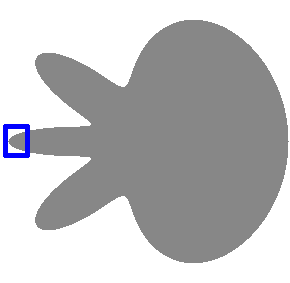
\includegraphics[scale=1.8]{figures/chapter5/cellular-grid/flower.png}
	}\hspace{40pt}%
	\subfloat[\label{}]{%	
	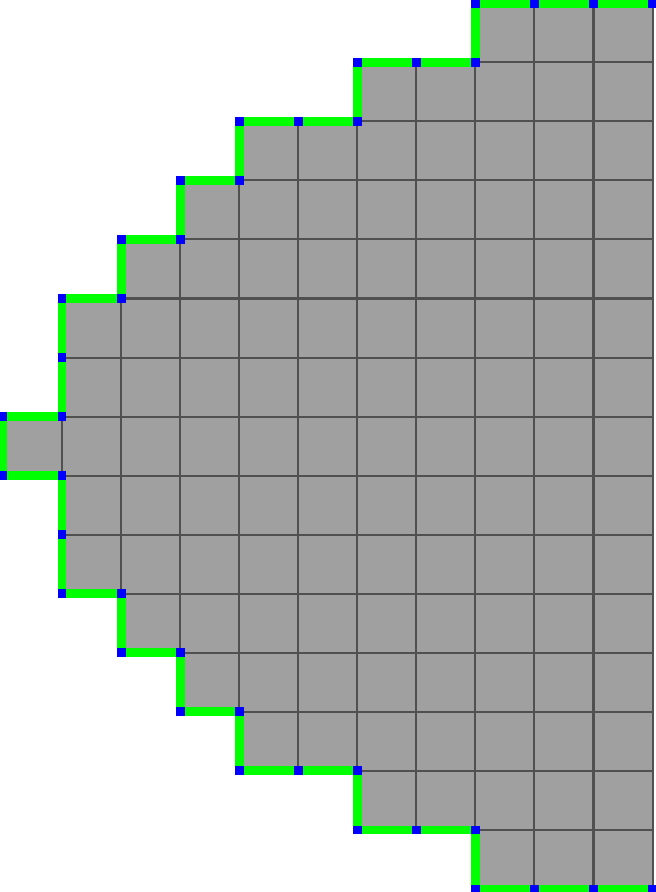
\includegraphics[scale=0.27]{figures/chapter5/cellular-grid/cellular-grid-illustration.pdf}
	}\hspace{40pt}%
	\subfloat[\label{}]{%
	\includegraphics[scale=0.035]{figures/chapter5/gcurves/distance-transform.pdf}
	}
	\caption{The flower shape in figure (a) and the cellular-grid model representation in (b) of the rectangle-bounded region. In figure (b), pixels are colored in gray, linels in green and pointels in blue. In figure (c), the blue pixels denotes a $3$-ring set.}
	\label{fig:cellular-grid-model}
\end{figure}


Consider the following set of neighbor candidates to $S$:
\begin{align*}
\mathcal{U}(S) = \{ D \; | D \subset R_1(S) \cup S \; \text{and} \; \text{$D$ is connected} \}.
\end{align*}


Such set can be extremely large and its complete exhaustion is prohibitively expensive.  Instead, we are going to use a subset of it.

Let $d_{S}:\Omega \rightarrow \mathbb{R}$ be the signed Euclidean distance transformation with respect to shape $S$. The value $d_S(p)$ gives the Euclidean distance between $p \notin S$ and the closest pixel in $S$. For points $p \in S$, $d_S(p)$ gives the distance between $p$ and the closest pixel not in $S$.


\begin{definition}{m-Ring Set}
Given a digital shape $S\in\Omega$, its signed distance transformation $d_S$ and natural number $m \neq 0$, the {\em $m$-ring set of $S$} is defined as
\begin{align*}
	R_m(S) &:= L_m \cup L_{-m},
\end{align*}
where
\begin{align*}
	L_m(S) &:= \left\{ \quad \begin{array}{cc}
		\left\{ p \in \Omega \; | \; m-1 < d_S(p) \leq m \right\} & , \quad m>0\\
		\left\{ p \in \Omega \; | \; m+1 > d_S(p) \geq m \right\} & , \quad m<0
		\end{array} \right.
\end{align*}
\end{definition}

\begin{definition}{$n$-neighborhood}

	Given a digital shape $S \in \Omega$, its $n$-neigh\-bor\-hood $\mathcal{N}_n(S)$ is defined as the set of digital shapes that can be built from $S$ by adding or removing a sequence of $k \in [0,n]$ connected pixels in $R_1(S)$.

\end{definition}




Algorithm~\ref{alg:local-search} describes the local combinatorial process and Figure~\ref{fig:local-comb-square-results} presents the evolution of four different shapes.


\begin{figure}[]
\center
\subfloat{
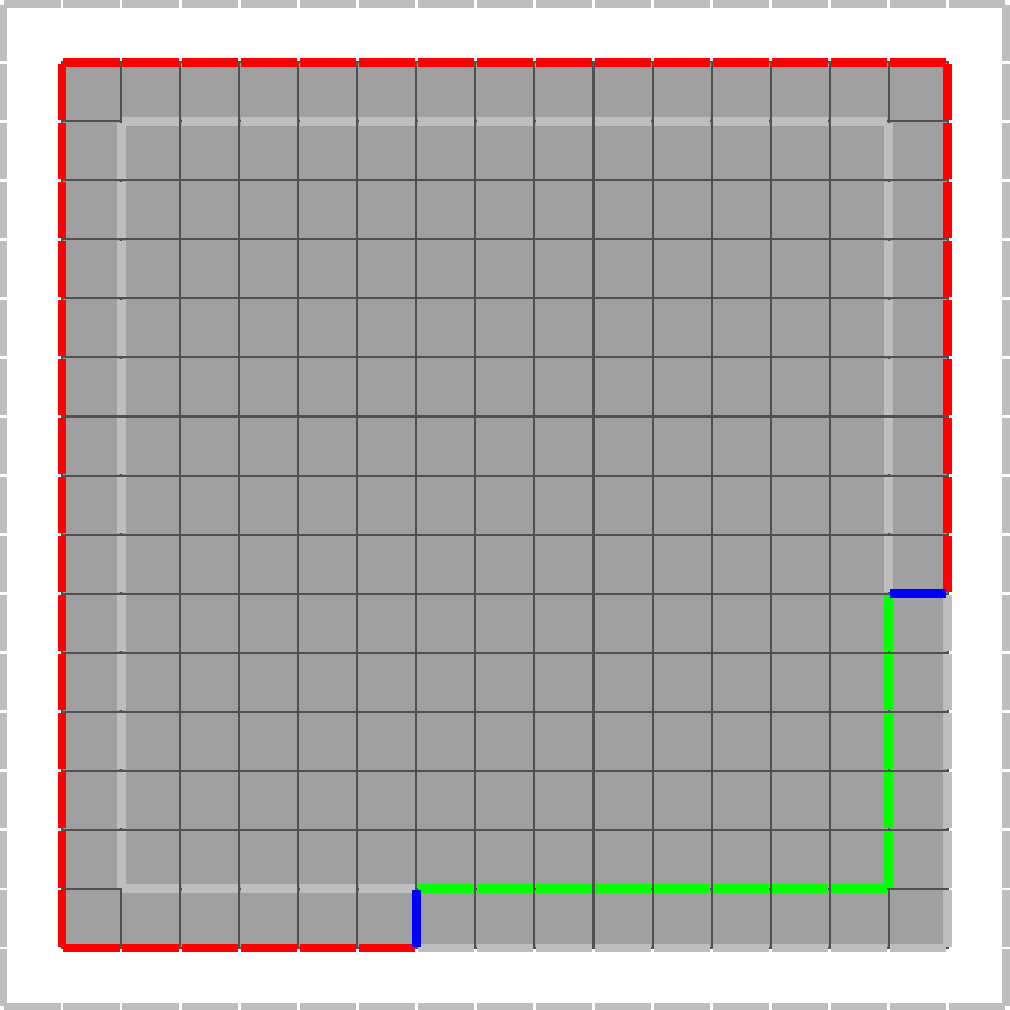
\includegraphics[scale=0.4]{figures/chapter5/gcurves/gc/main-inner.pdf}
}\hspace{1em}%
\subfloat{
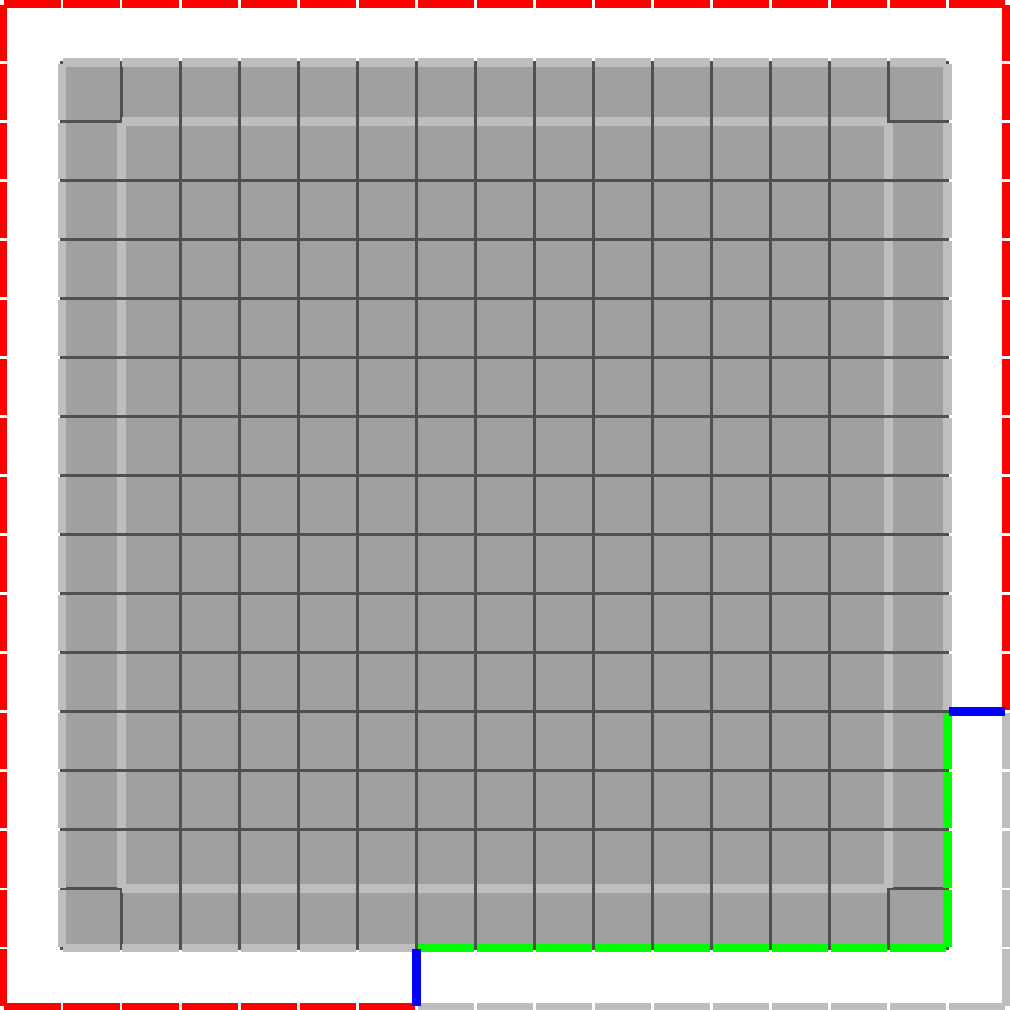
\includegraphics[scale=0.4]{figures/chapter5/gcurves/gc/main-outer.pdf}
}\hspace{1em}\\[1em]
\subfloat{
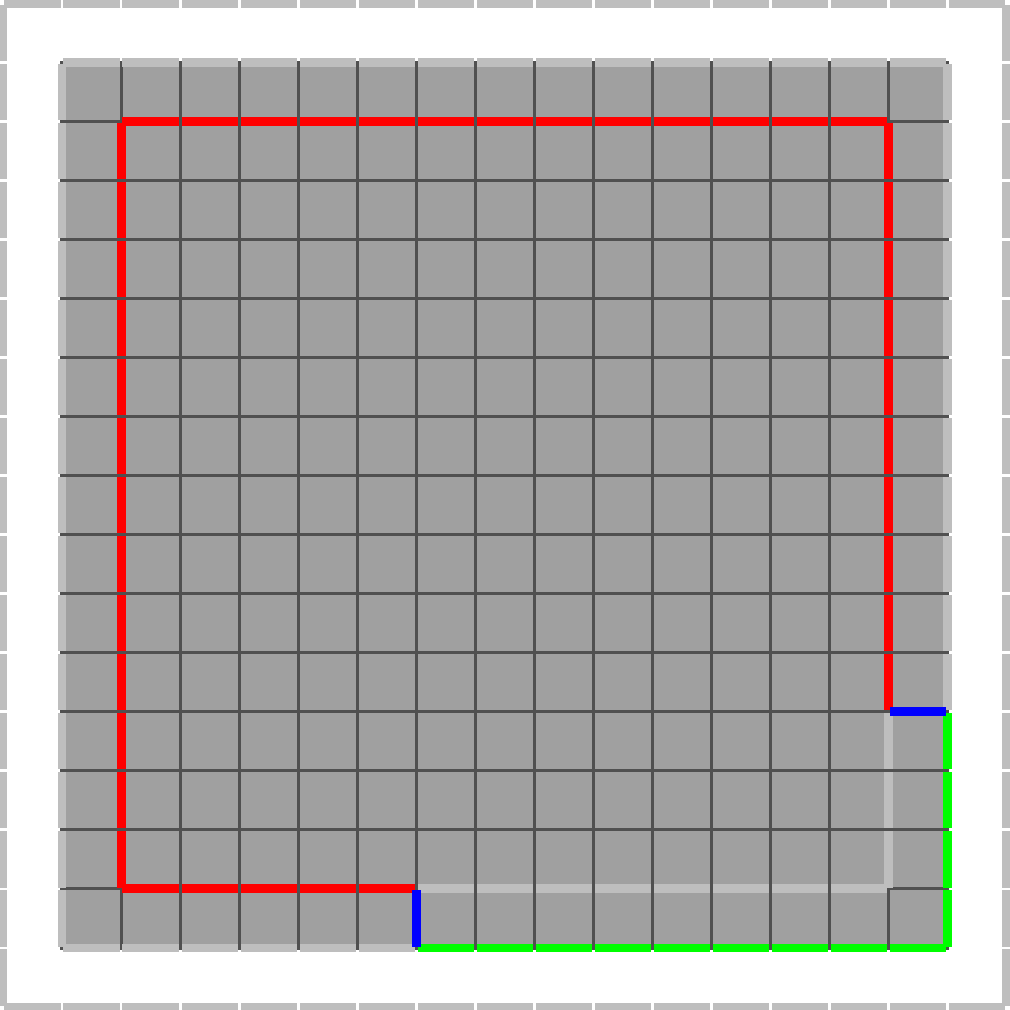
\includegraphics[scale=0.4]{figures/chapter5/gcurves/gc/inner-main.pdf}
}\hspace{1em}%
\subfloat{
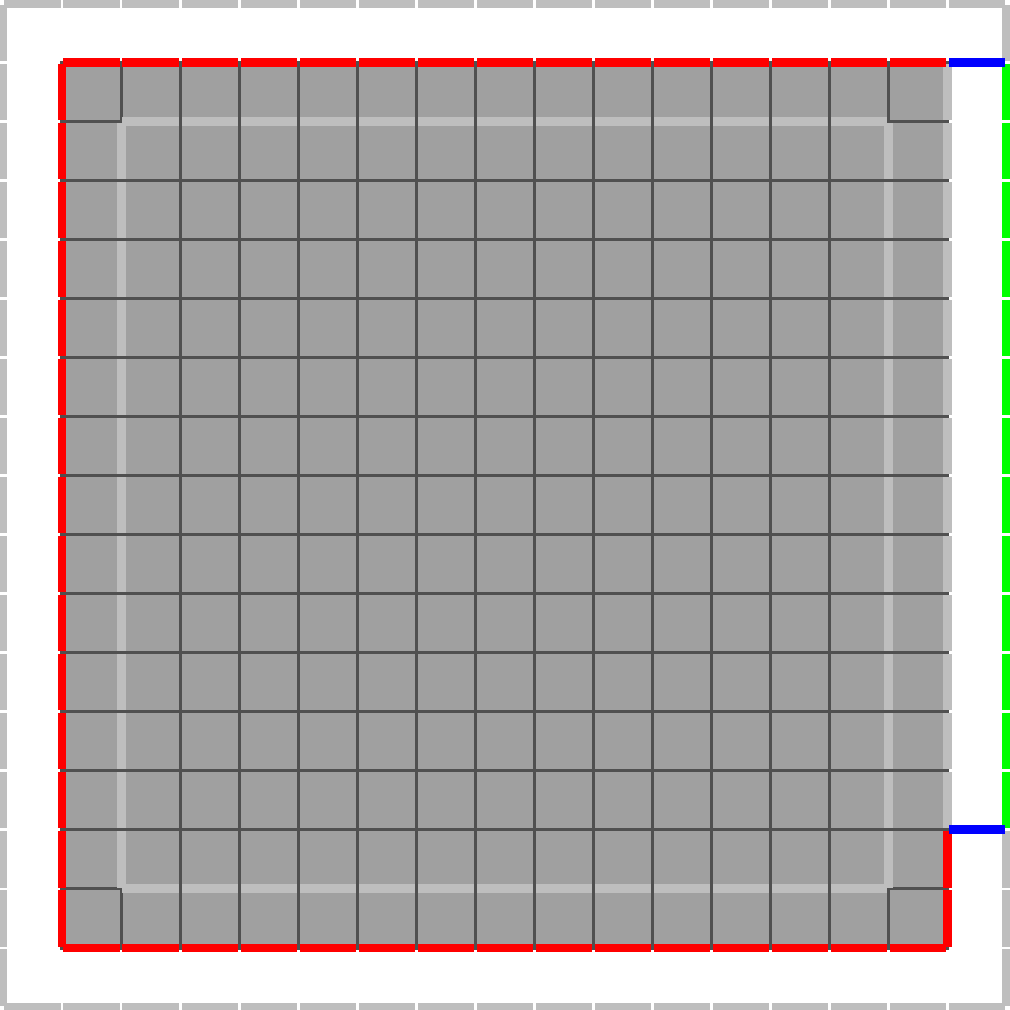
\includegraphics[scale=0.4]{figures/chapter5/gcurves/gc/outer-main.pdf}
}\hspace{1em}%
\caption{Members of $\mathcal{N}_{11}$ for the square shape.}
\end{figure}


\begin{algorithm}[H]
 \SetKwData{It}{i}
 \SetKwData{MIt}{maxIt}
 \SetKwData{Delta}{delta}
 \SetKwData{Best}{best} 
 \SetKwInOut{Input}{input}\SetKwInOut{Output}{output}
 
 \Input{A digital set $S$ and the maximum number of iterations \MIt}
 \BlankLine
 $i \longleftarrow 0$\;	
 $S^{(0)} \longleftarrow S$\;
 \While{ $k < \log_2{|\partial S^{(i)}|}$ \bf{and} \It $<$ \MIt }
 {
	$n \longleftarrow |\partial S|/(3 \cdot 2^k)$\; 
 
 
  	\For{$ X \in \mathcal{N}_n(S^{(i)}) \cup \mathcal{N}_{2n}(S^{(i)}) \cup \mathcal{N}_{3n}(S^{(i)}) $}
	{
		\If{ $\hat{E}(X)$ $<$ $\hat{E}(X^\star)$ }
		{
			$X^\star \longleftarrow X$\; 
		}	
	}
	\Delta $\longleftarrow$ $\hat{E}(S^{(i-1)}) - \hat{E}(S^{(i)})$\;	
	
	\If{ \Delta $=0$ }
	{
		$k \longleftarrow k+1$\; 
	}		
	\Else{
		$k \longleftarrow 1$\;	
		$S^{(i)} \longleftarrow X^\star$\;
		\It $\longleftarrow$ \It $+1$\;		
	}
	
 }
 \label{alg:local-search} 
 \caption{Local combinatorial optimization for elastica minimization.}
\end{algorithm}

\begin{figure}[]
\center
\subfloat{
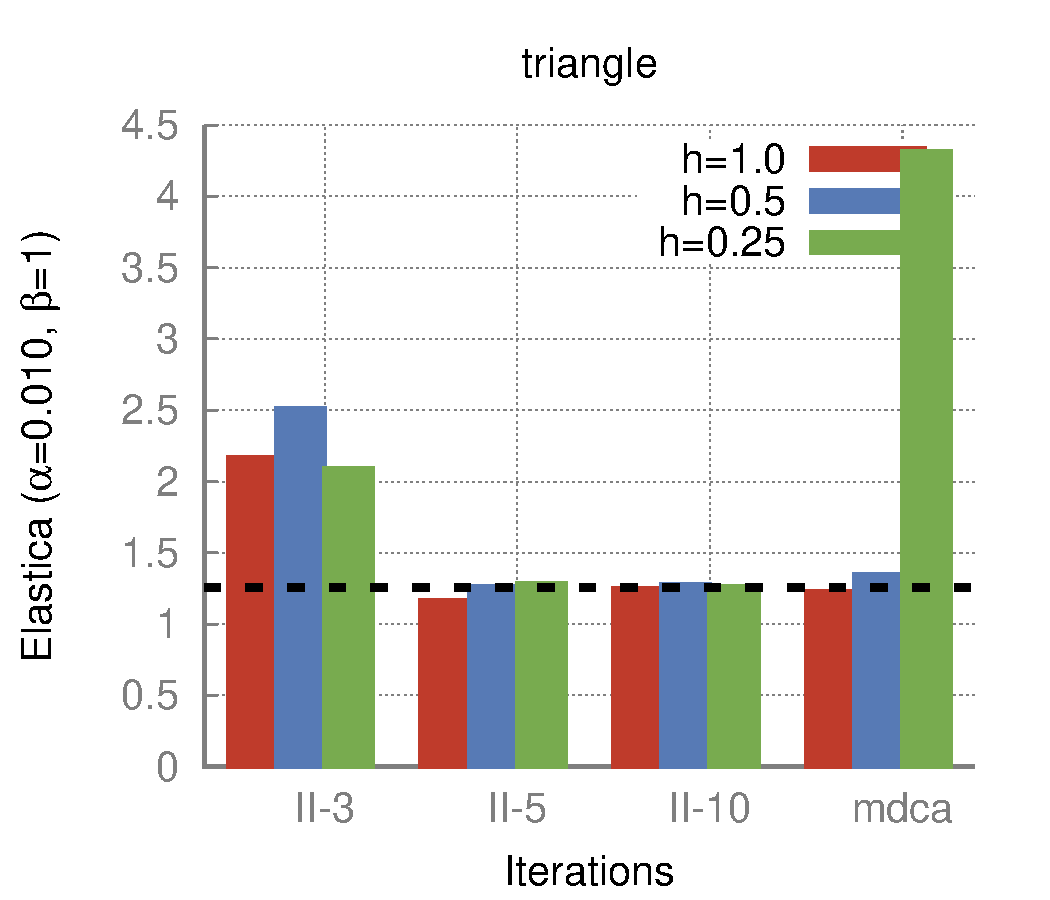
\includegraphics[scale=0.4]{figures/chapter5/flow/plots/bars/length_pen_0.01000/triangle.pdf}
}\hspace{1em}%
\subfloat{
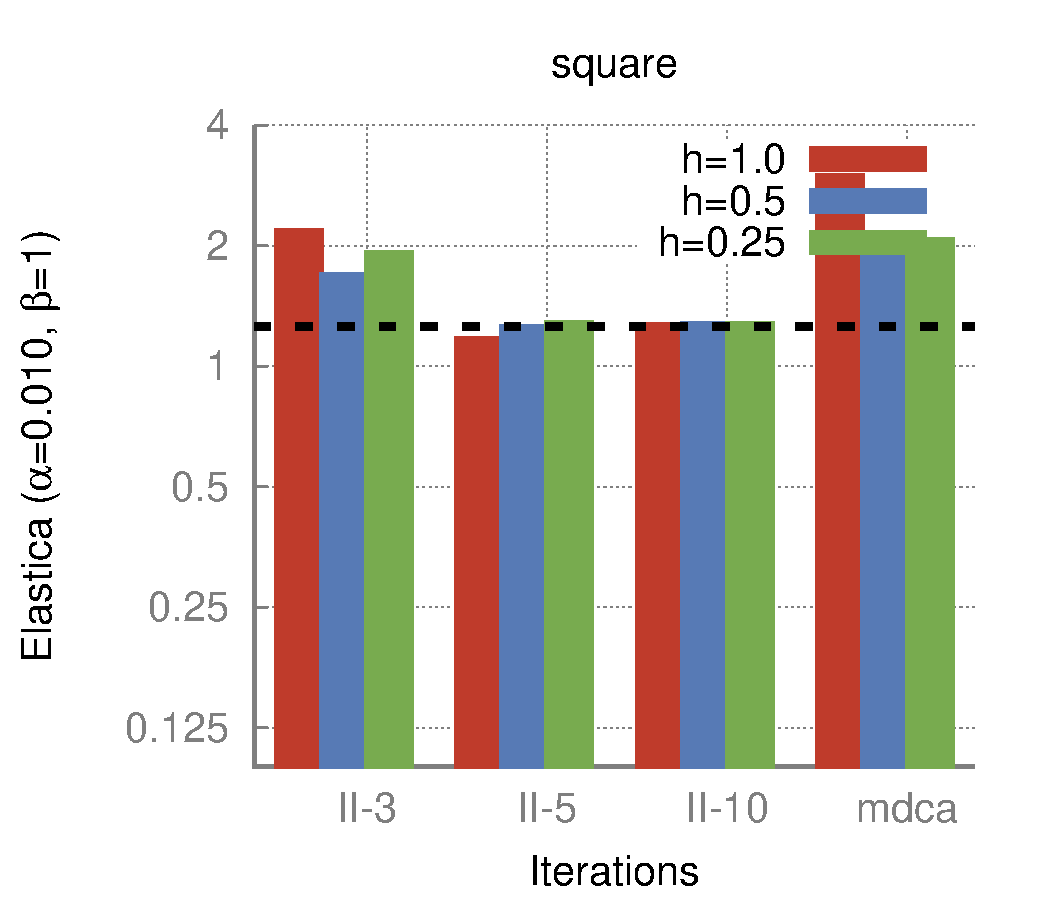
\includegraphics[scale=0.4]{figures/chapter5/flow/plots/bars/length_pen_0.01000/square.pdf}
}\hspace{1em}%
\subfloat{
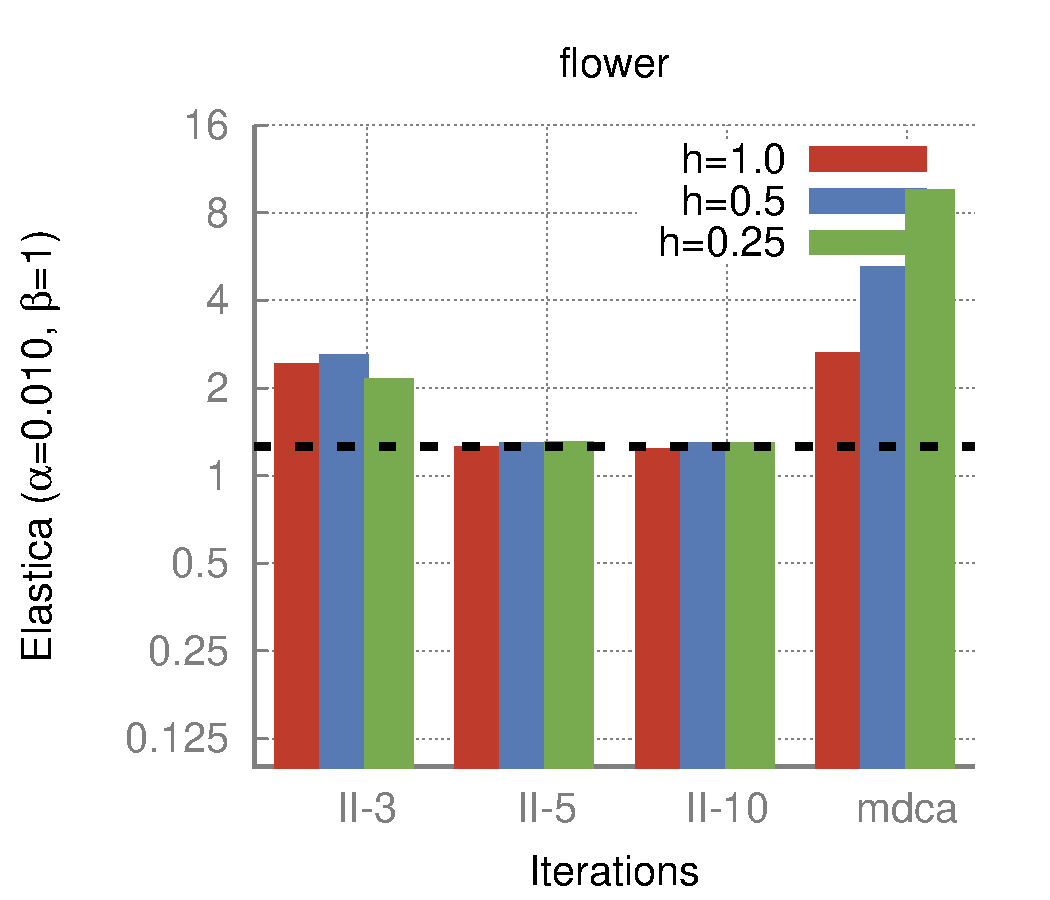
\includegraphics[scale=0.4]{figures/chapter5/flow/plots/bars/length_pen_0.01000/flower.pdf}
}\hspace{1em}%
\subfloat{
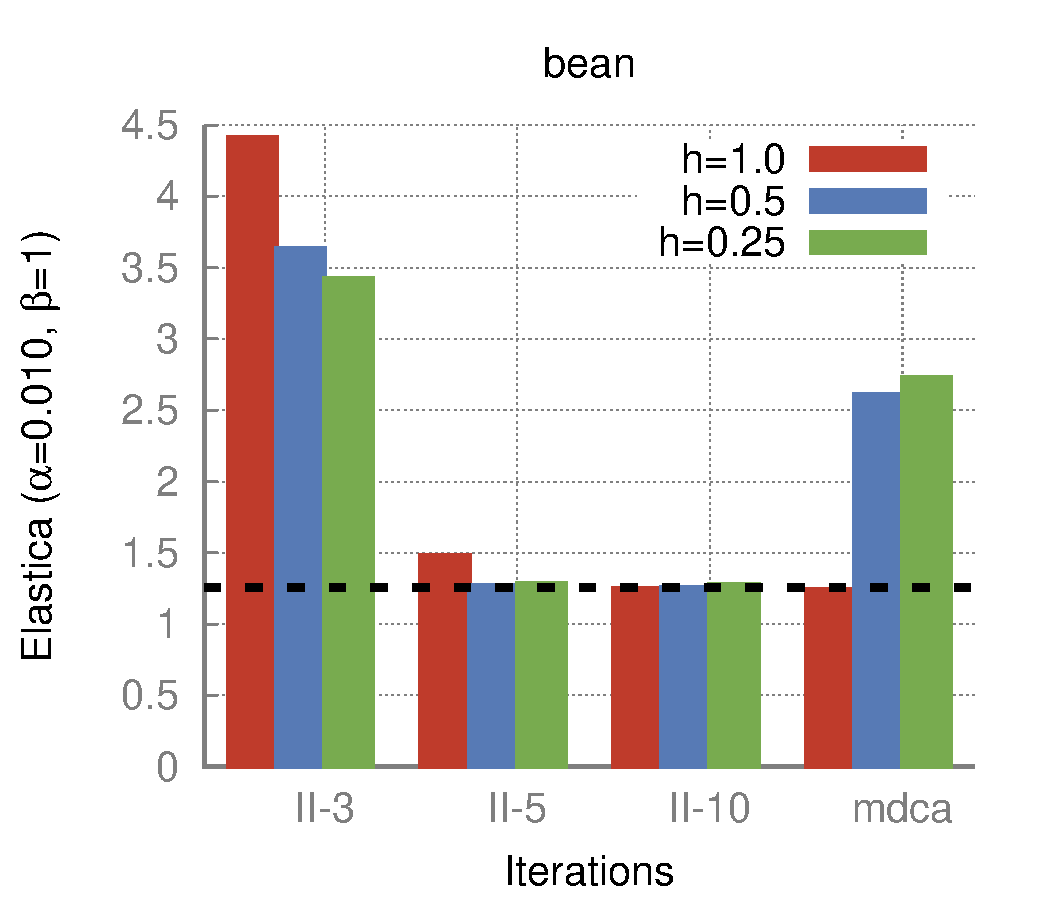
\includegraphics[scale=0.4]{figures/chapter5/flow/plots/bars/length_pen_0.01000/bean.pdf}
}\hspace{1em}%
\subfloat{
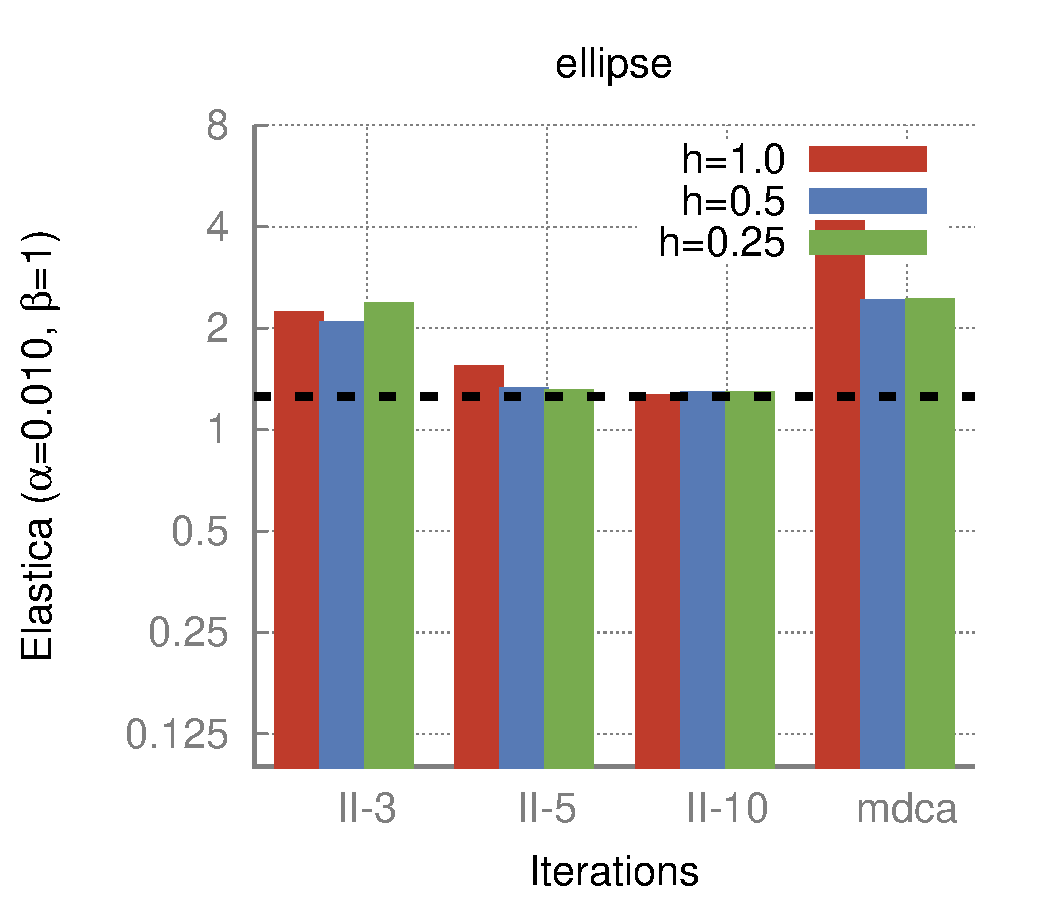
\includegraphics[scale=0.4]{figures/chapter5/flow/plots/bars/length_pen_0.01000/ellipse.pdf}
}\hspace{1em}%
\subfloat{
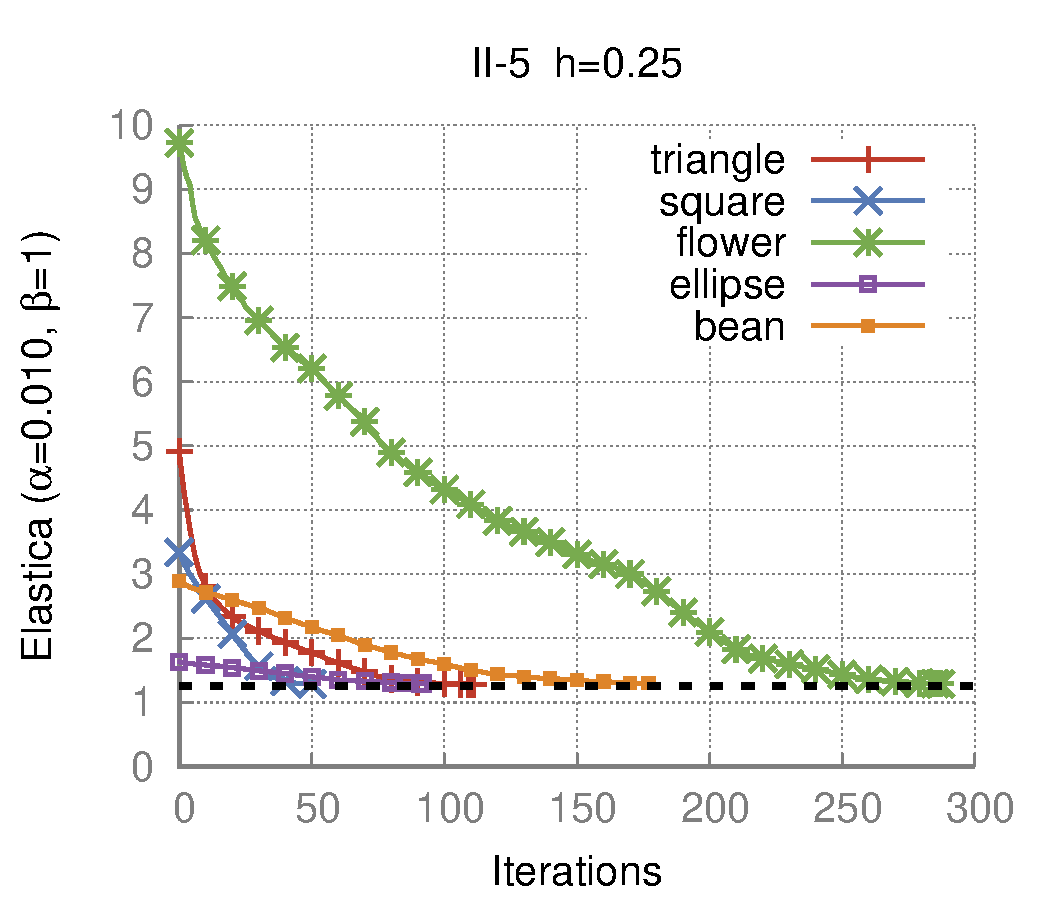
\includegraphics[scale=0.4]{figures/chapter5/flow/plots/summary/lp_0.01/summary-ii5.pdf}
}%
\caption{Minimum value attained for the digial elastica ($\alpha=0.01, \beta=1$) in comparisson with the global optimium (dashed line) for different curvature estimators and in different scales. The last figure summarizes the digital elastica evolution value for all shapes using grid step $h=0.25$.}
\label{fig:local-comb-estimators-plots-lp001}
\end{figure}

\begin{figure}[]
\center
\subfloat{
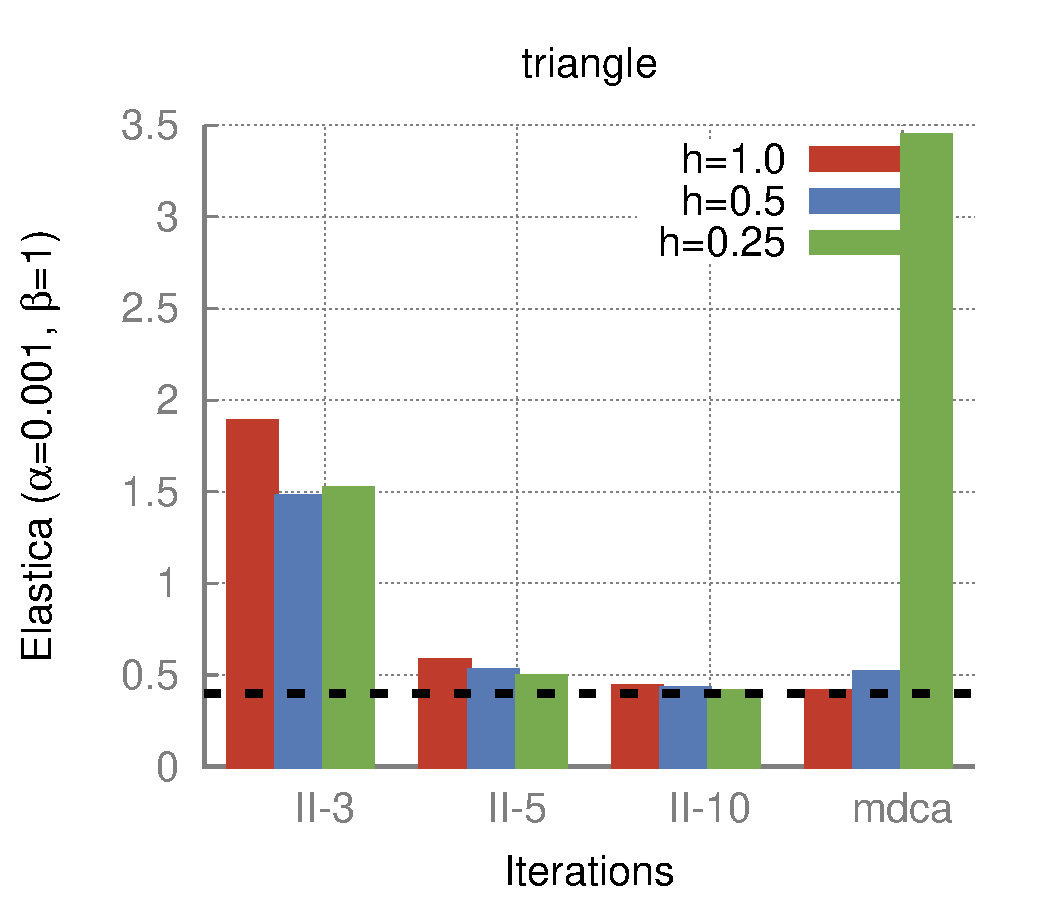
\includegraphics[scale=0.4]{figures/chapter5/flow/plots/bars/length_pen_0.00100/triangle.pdf}
}\hspace{1em}%
\subfloat{
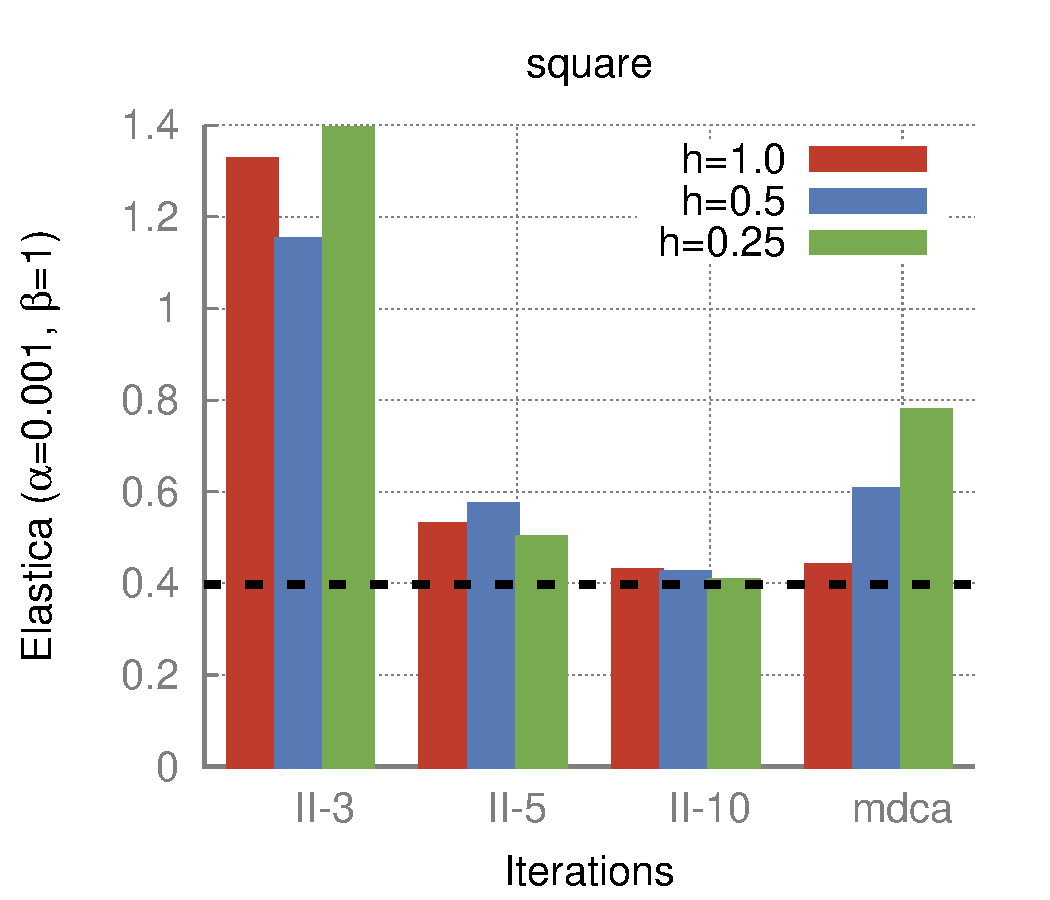
\includegraphics[scale=0.4]{figures/chapter5/flow/plots/bars/length_pen_0.00100/square.pdf}
}\hspace{1em}%
\subfloat{
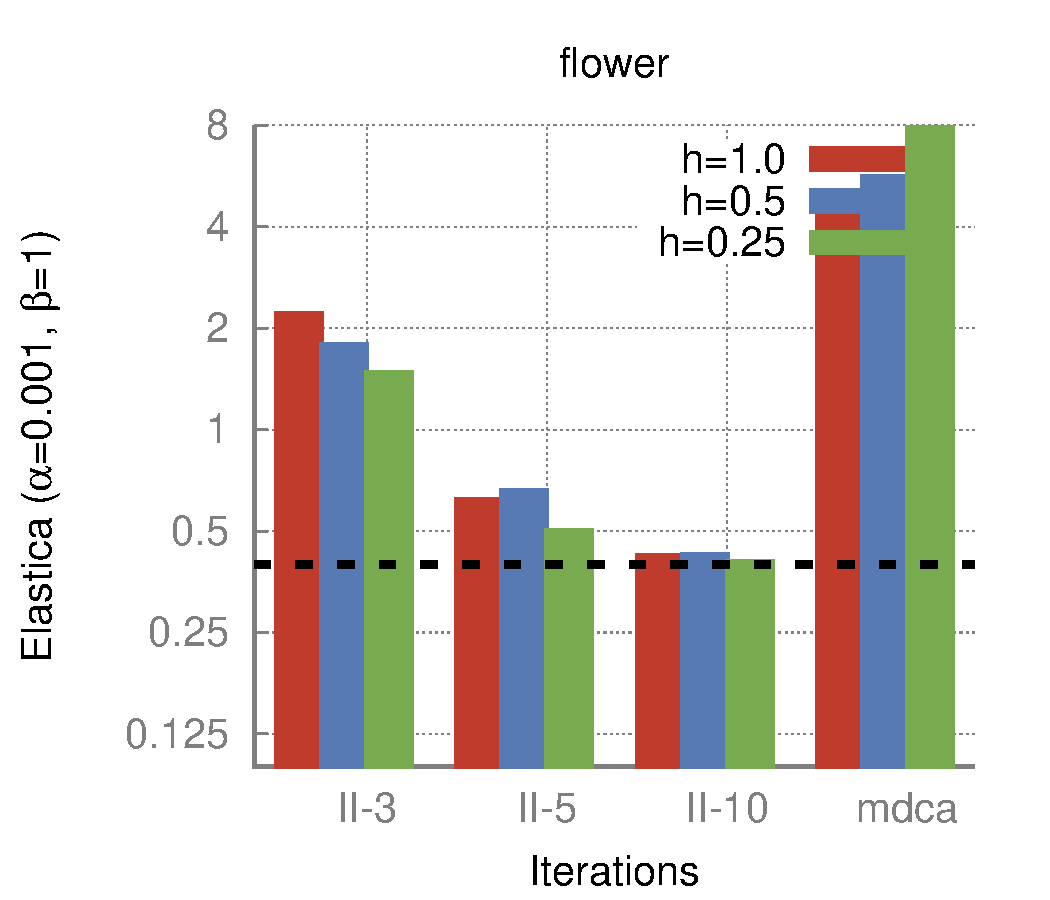
\includegraphics[scale=0.4]{figures/chapter5/flow/plots/bars/length_pen_0.00100/flower.pdf}
}\hspace{1em}%
\subfloat{
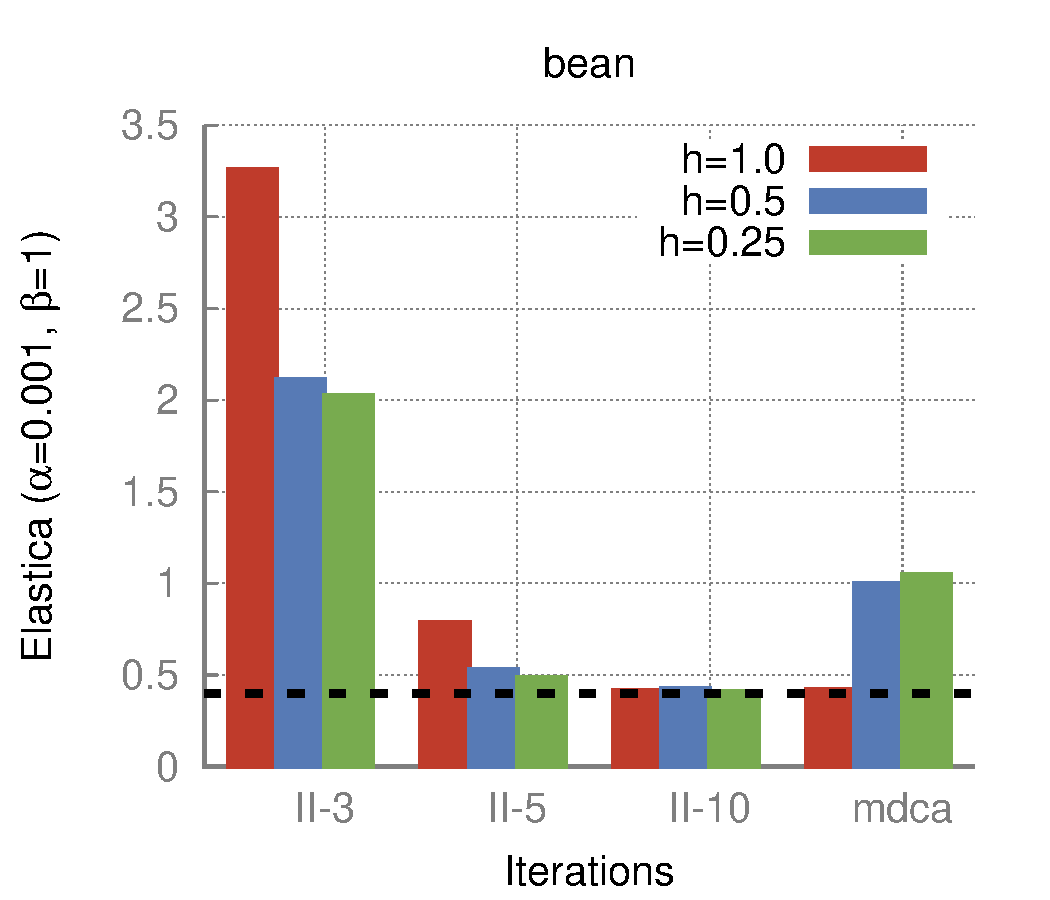
\includegraphics[scale=0.4]{figures/chapter5/flow/plots/bars/length_pen_0.00100/bean.pdf}
}\hspace{1em}%
\subfloat{
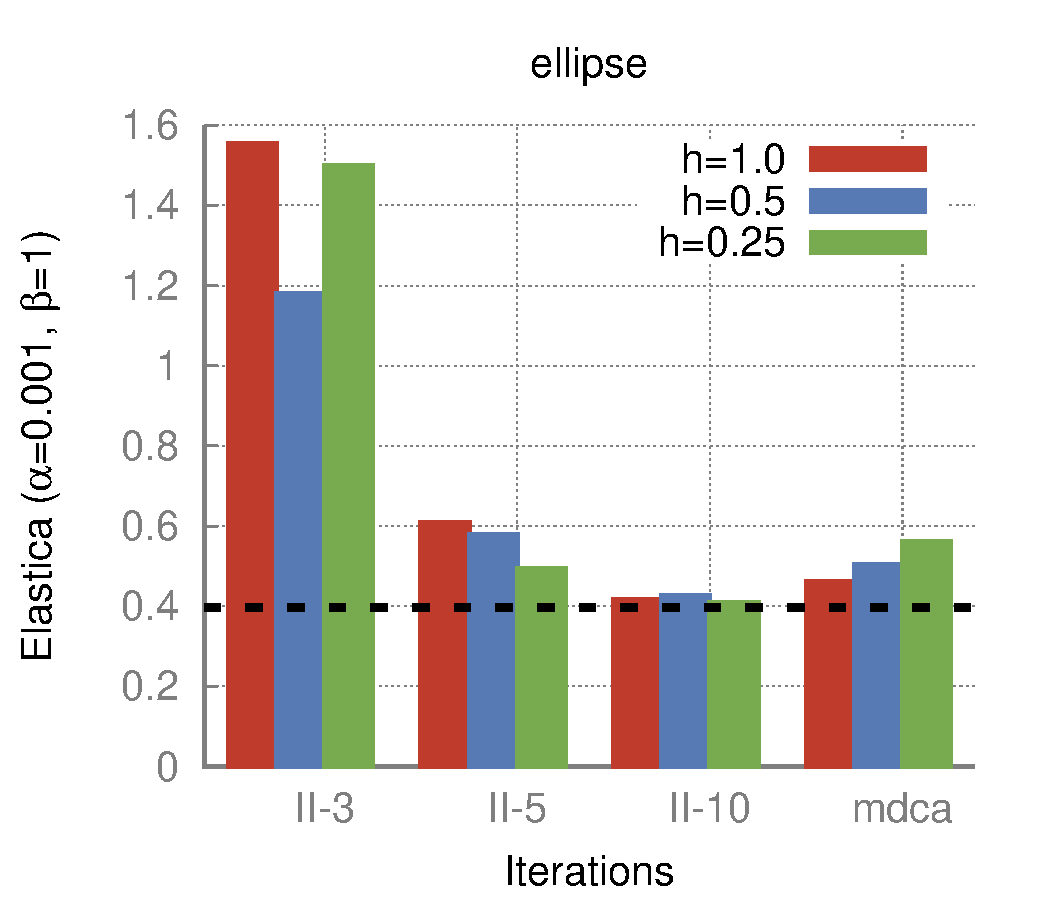
\includegraphics[scale=0.4]{figures/chapter5/flow/plots/bars/length_pen_0.00100/ellipse.pdf}
}\hspace{1em}%
\subfloat{
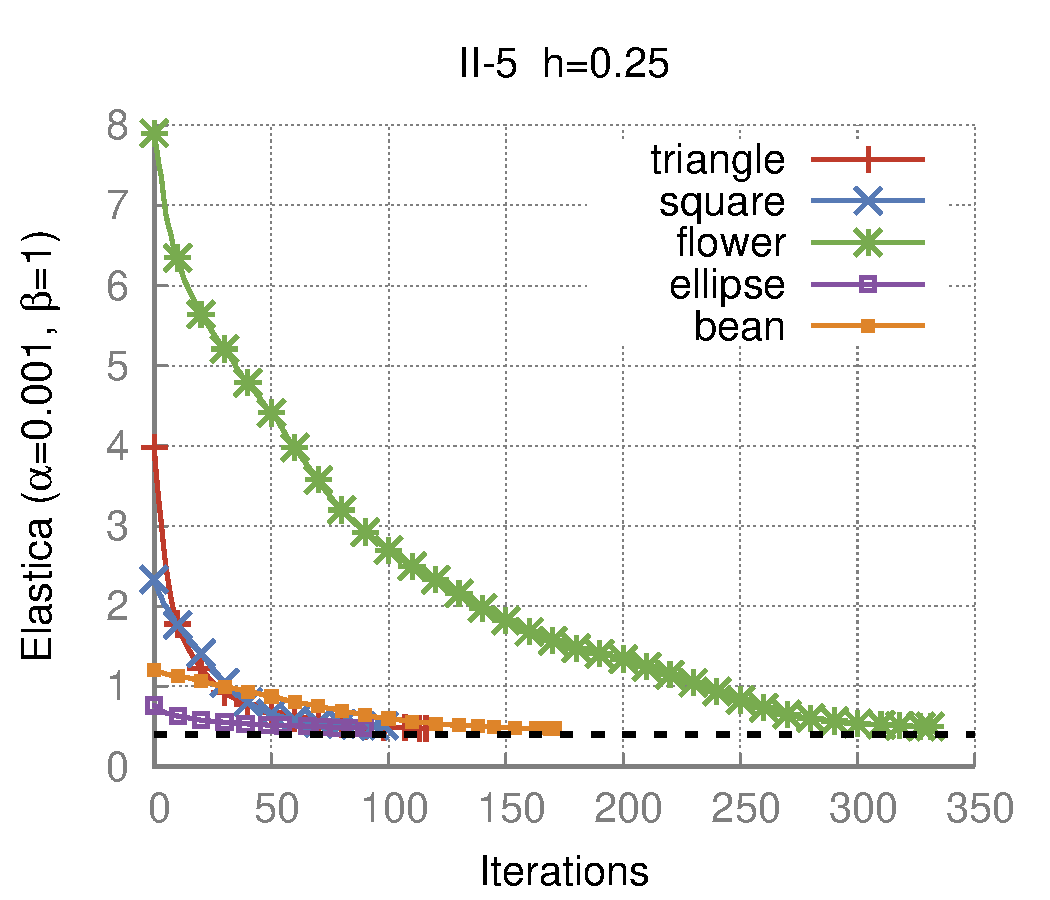
\includegraphics[scale=0.4]{figures/chapter5/flow/plots/summary/lp_0.001/summary-ii5.pdf}
}%
\caption{Minimum value attained for the digial elastica ($\alpha=0.001, \beta=1$) in comparisson with the global optimium (dashed line) for different curvature estimators and in different scales. The last figure summarizes the digital elastica evolution value for all shapes using grid step $h=0.25$.}
\label{fig:local-comb-estimators-plots-lp0001}
\end{figure}


\begin{figure}[hp!]
	\center
	\begin{tabular}{ccc}
		$h=1.0$ & $h=0.5$ & $h=0.25$ \\[2em]
	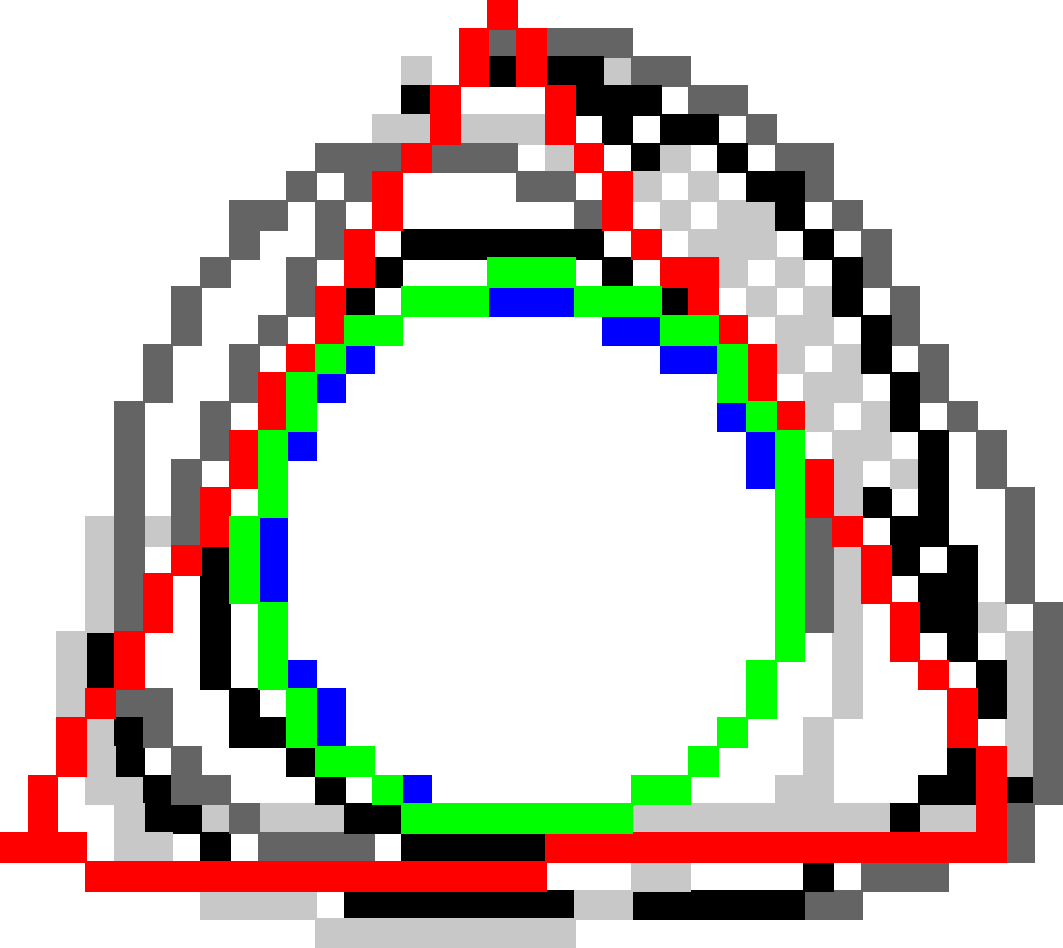
\includegraphics[scale=0.185]{figures/chapter5/flow/triangle/radius_5/ii/elastica/len_pen_0.01000/jonctions_1/best/gs_1.00000/summary.pdf} &
	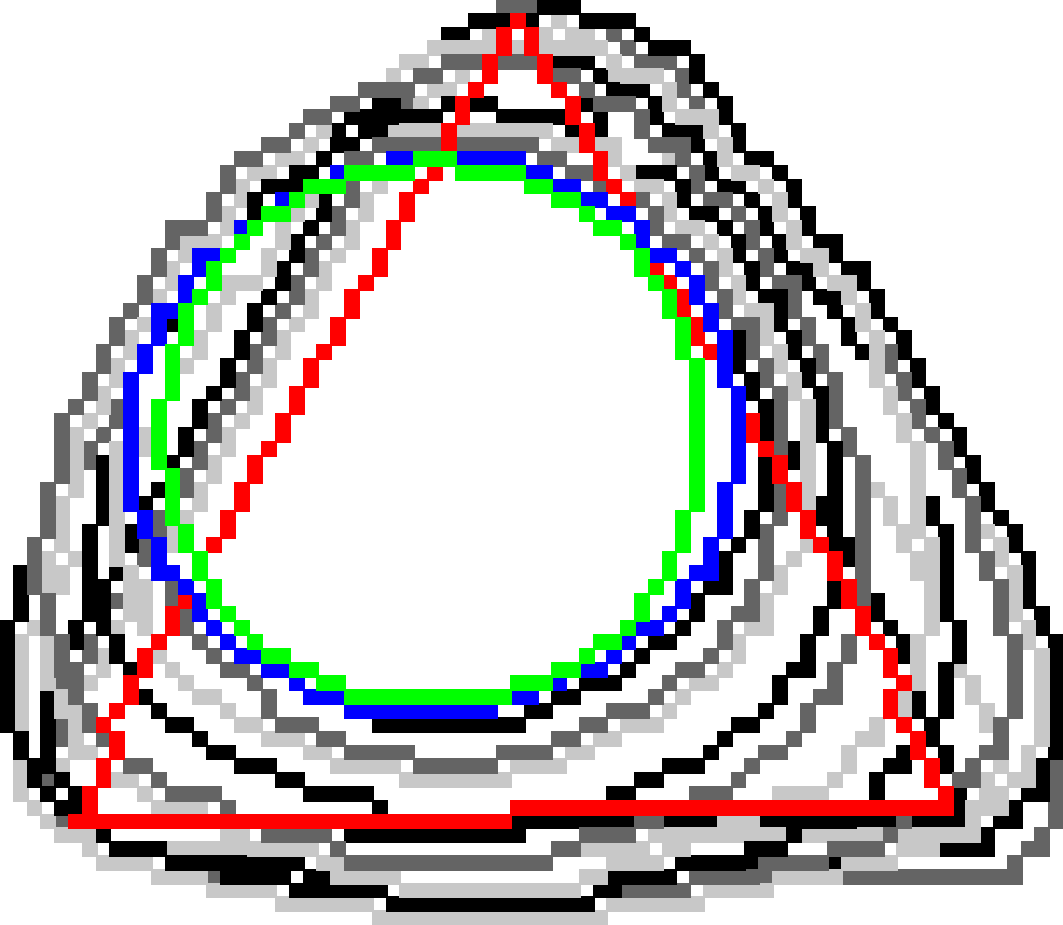
\includegraphics[scale=0.185]{figures/chapter5/flow/triangle/radius_5/ii/elastica/len_pen_0.01000/jonctions_1/best/gs_0.50000/summary.pdf} &
	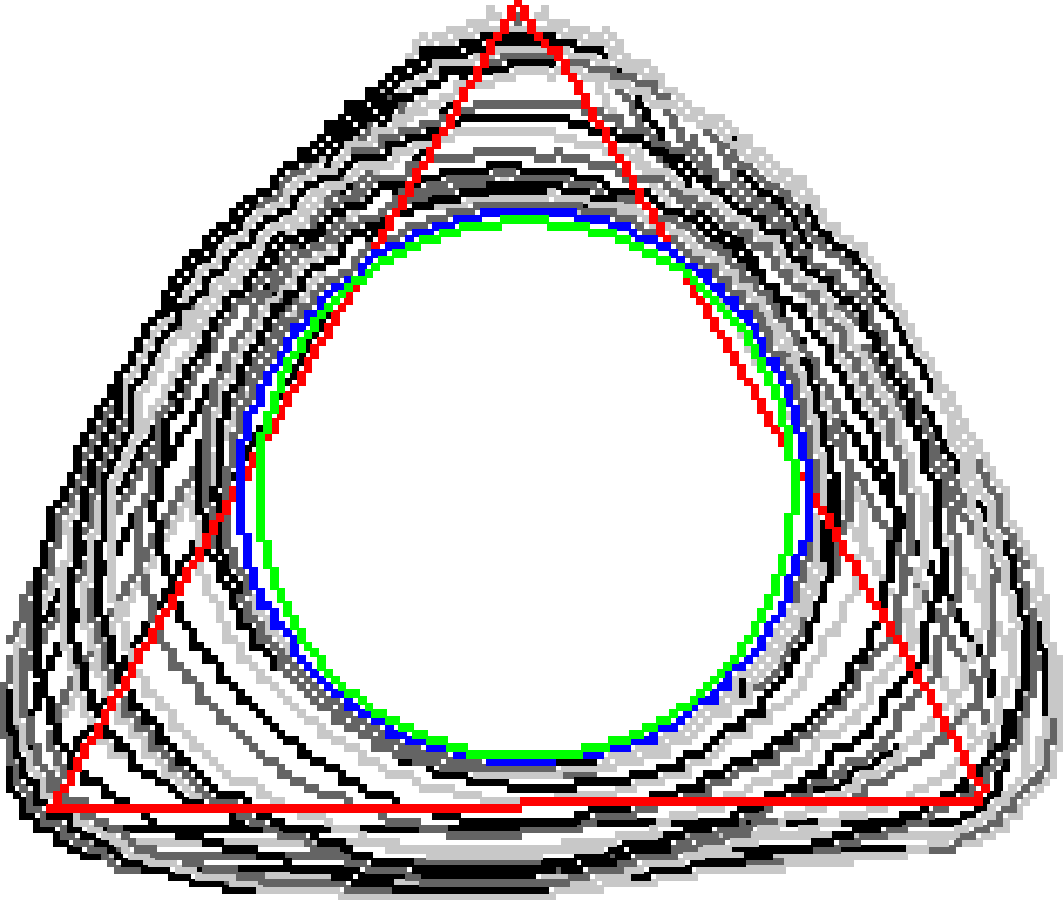
\includegraphics[scale=0.185]{figures/chapter5/flow/triangle/radius_5/ii/elastica/len_pen_0.01000/jonctions_1/best/gs_0.25000/summary.pdf}\\[2em]
		
	
\includegraphics[scale=0.17]{figures/chapter5/flow/square/radius_5/ii/elastica/len_pen_0.01000/jonctions_1/best/gs_1.00000/summary.pdf} &
	
	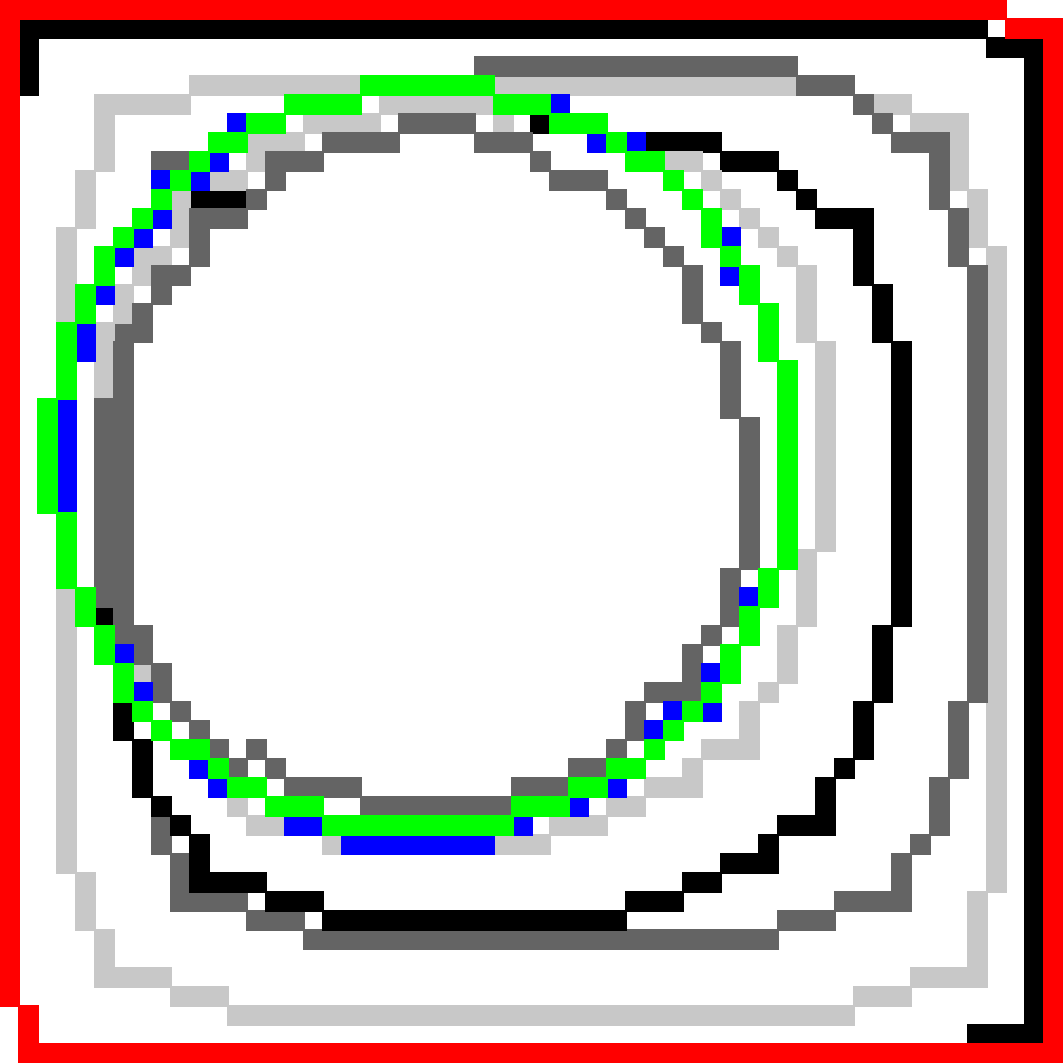
\includegraphics[scale=0.17]{figures/chapter5/flow/square/radius_5/ii/elastica/len_pen_0.01000/jonctions_1/best/gs_0.50000/summary.pdf} &	
	
	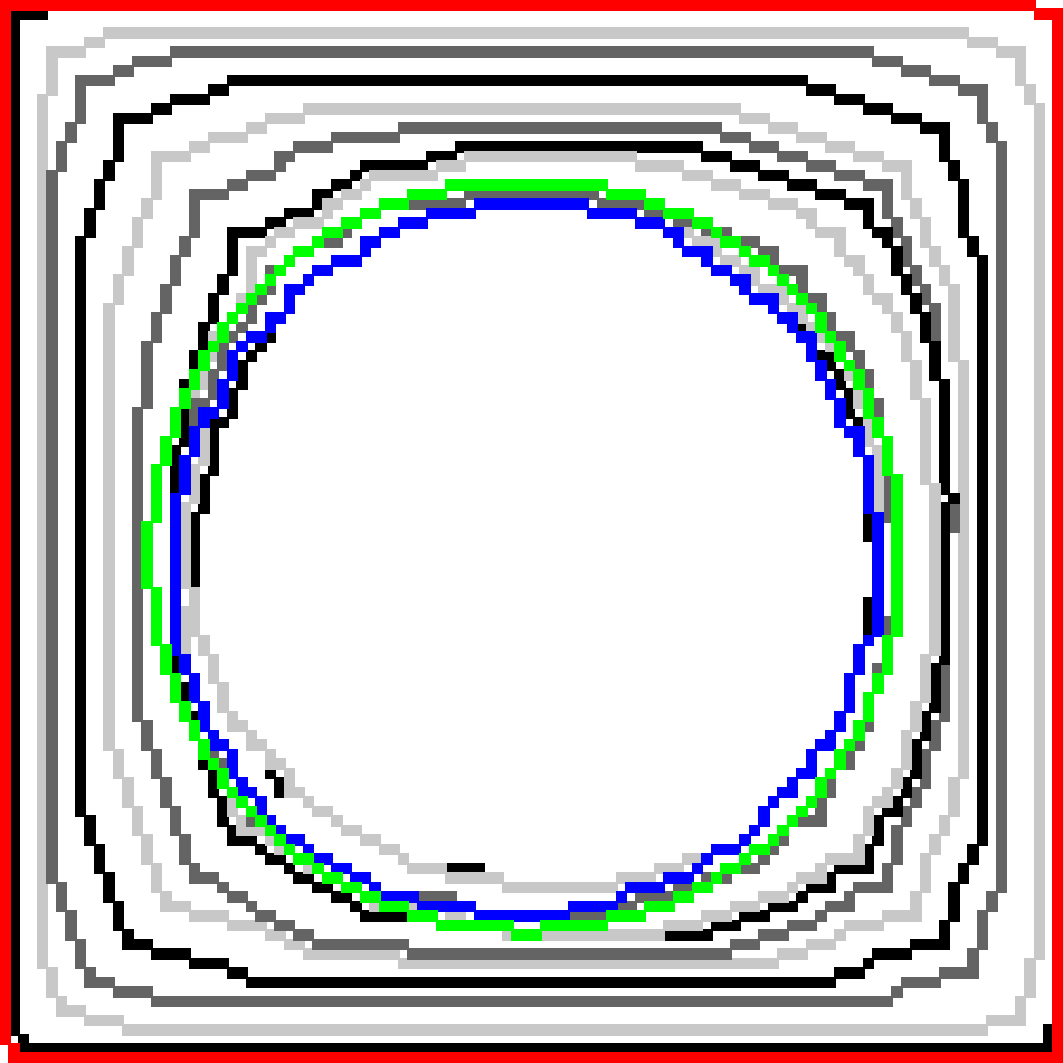
\includegraphics[scale=0.17]{figures/chapter5/flow/square/radius_5/ii/elastica/len_pen_0.01000/jonctions_1/best/gs_0.25000/summary.pdf}\\[2em]
	
	
	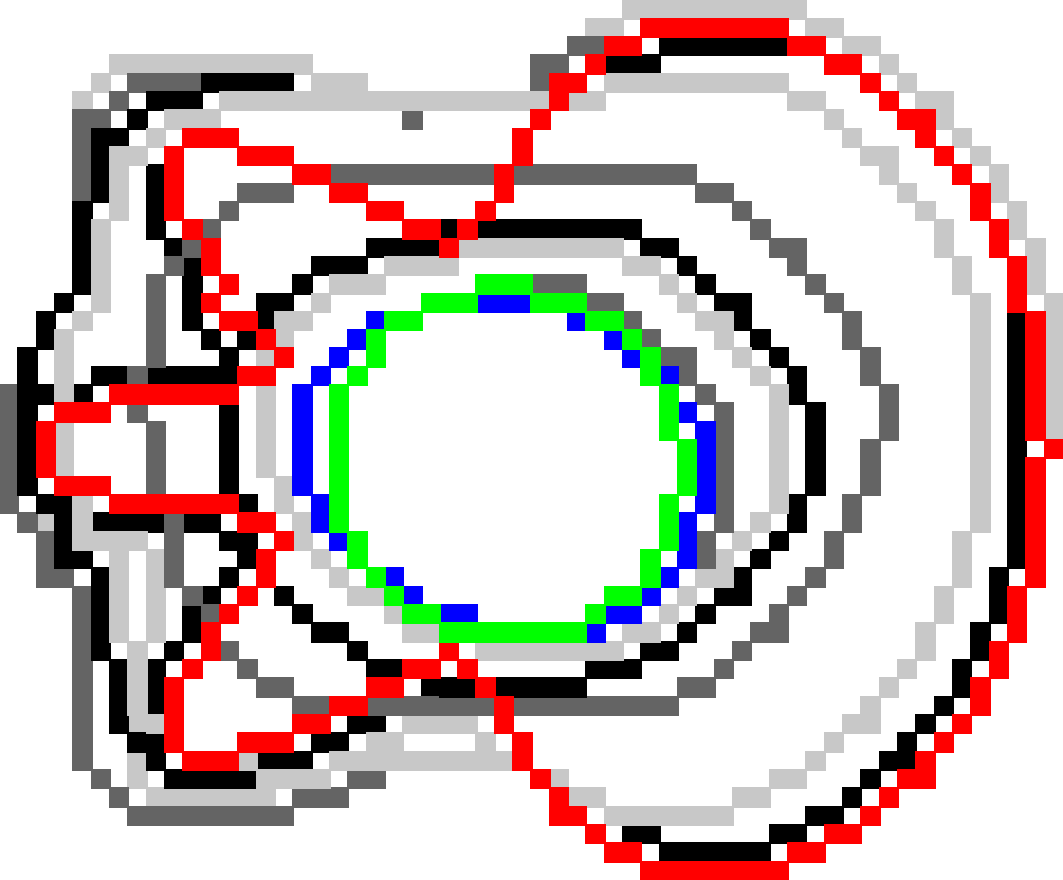
\includegraphics[scale=0.25]{figures/chapter5/flow/flower/radius_5/ii/elastica/len_pen_0.01000/jonctions_1/best/gs_1.00000/summary.pdf} &		
	
	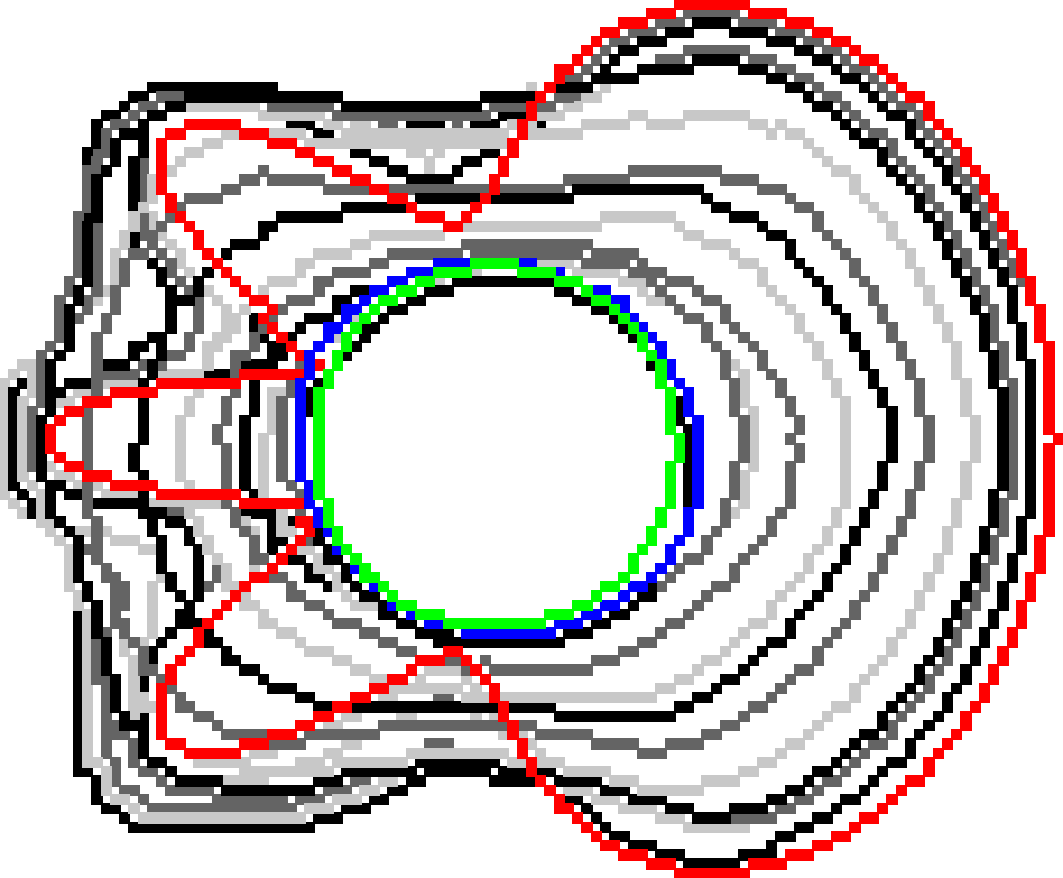
\includegraphics[scale=0.25]{figures/chapter5/flow/flower/radius_5/ii/elastica/len_pen_0.01000/jonctions_1/best/gs_0.50000/summary.pdf} &

	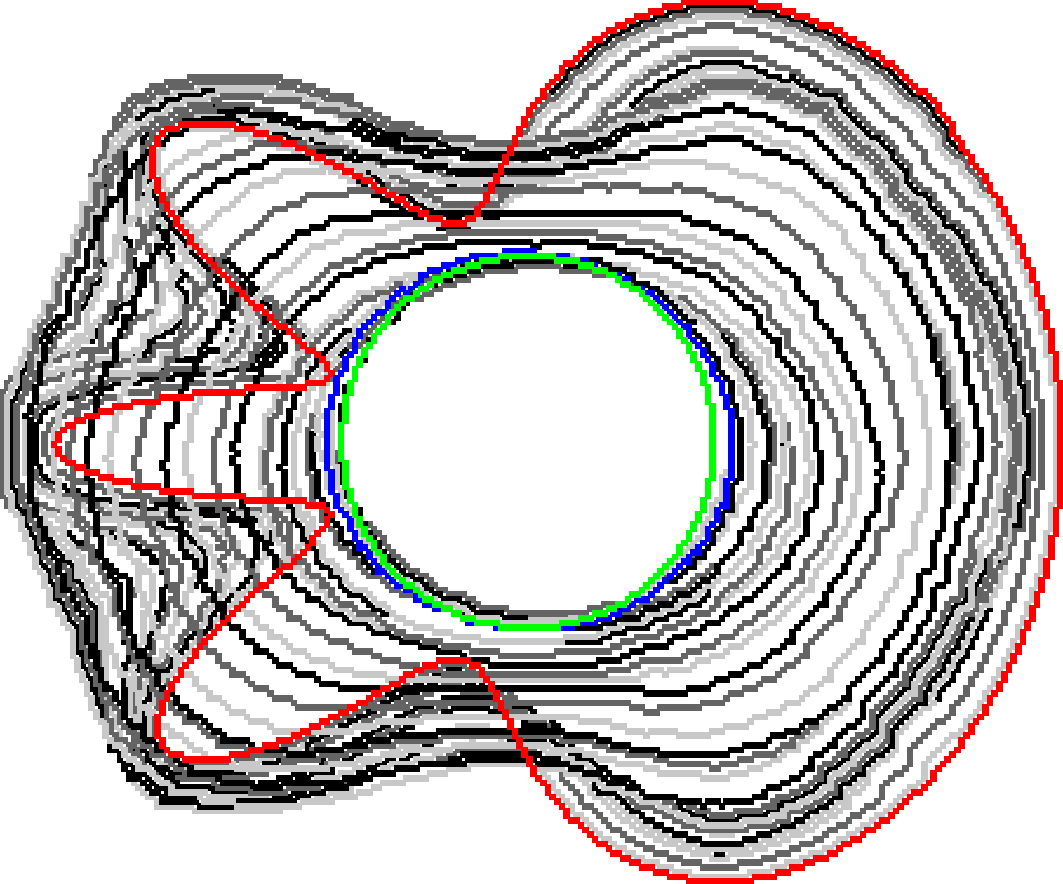
\includegraphics[scale=0.25]{figures/chapter5/flow/flower/radius_5/ii/elastica/len_pen_0.01000/jonctions_1/best/gs_0.25000/summary.pdf}\\[2em]	
	
	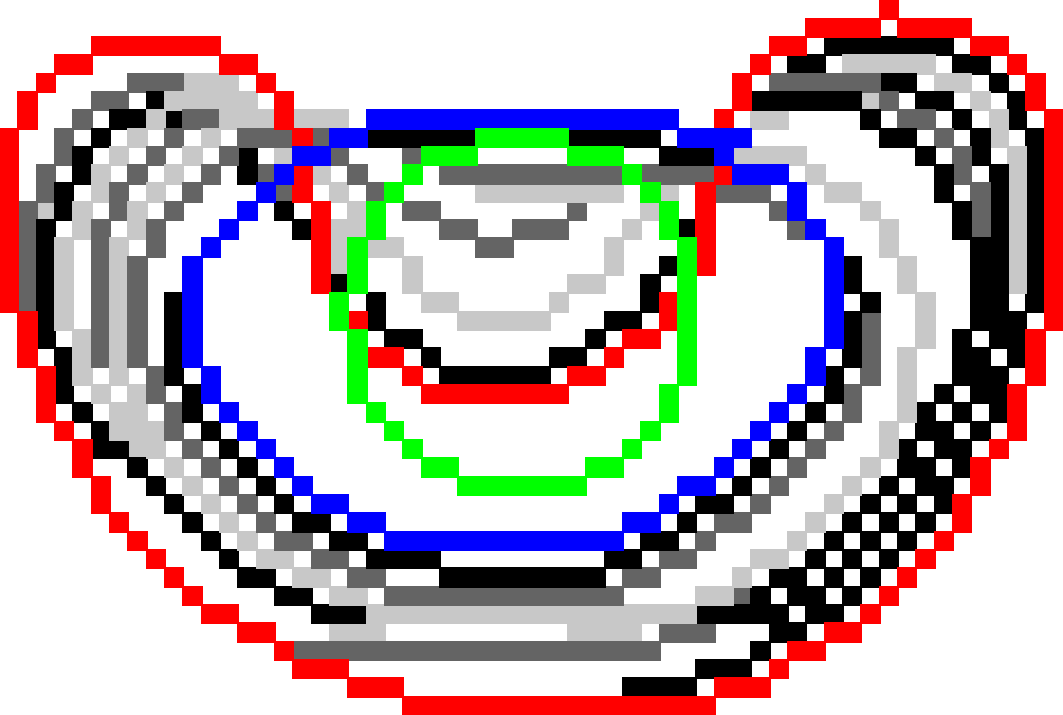
\includegraphics[scale=0.25]{figures/chapter5/flow/bean/radius_5/ii/elastica/len_pen_0.01000/jonctions_1/best/gs_1.00000/summary.pdf} &	 
	
	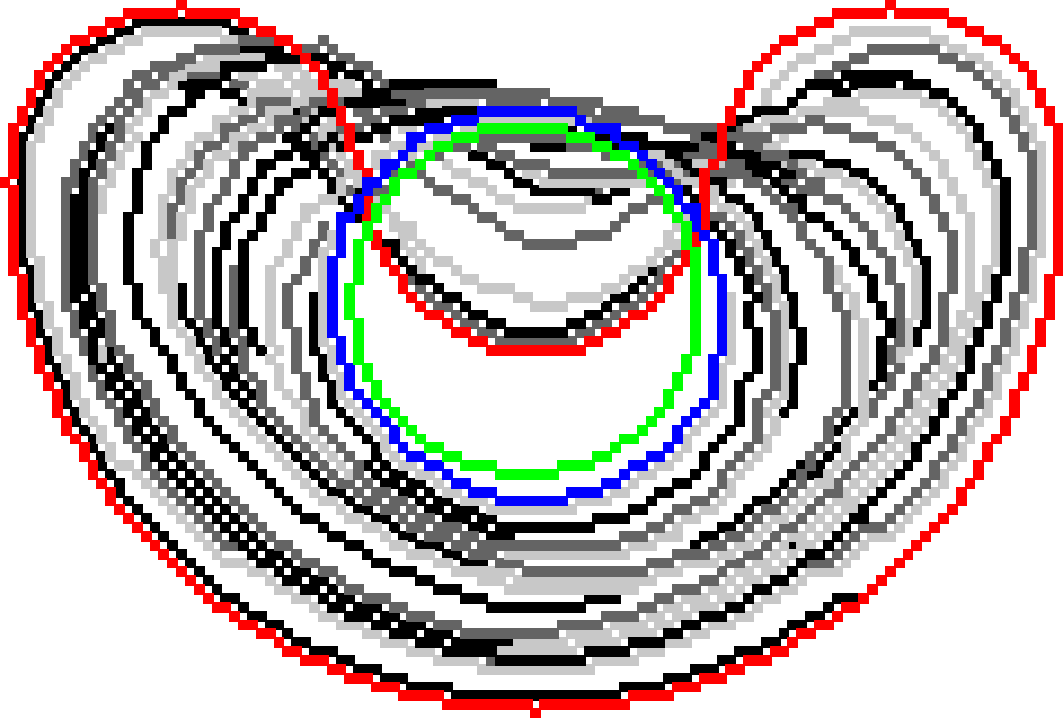
\includegraphics[scale=0.25]{figures/chapter5/flow/bean/radius_5/ii/elastica/len_pen_0.01000/jonctions_1/best/gs_0.50000/summary.pdf} &	
	
	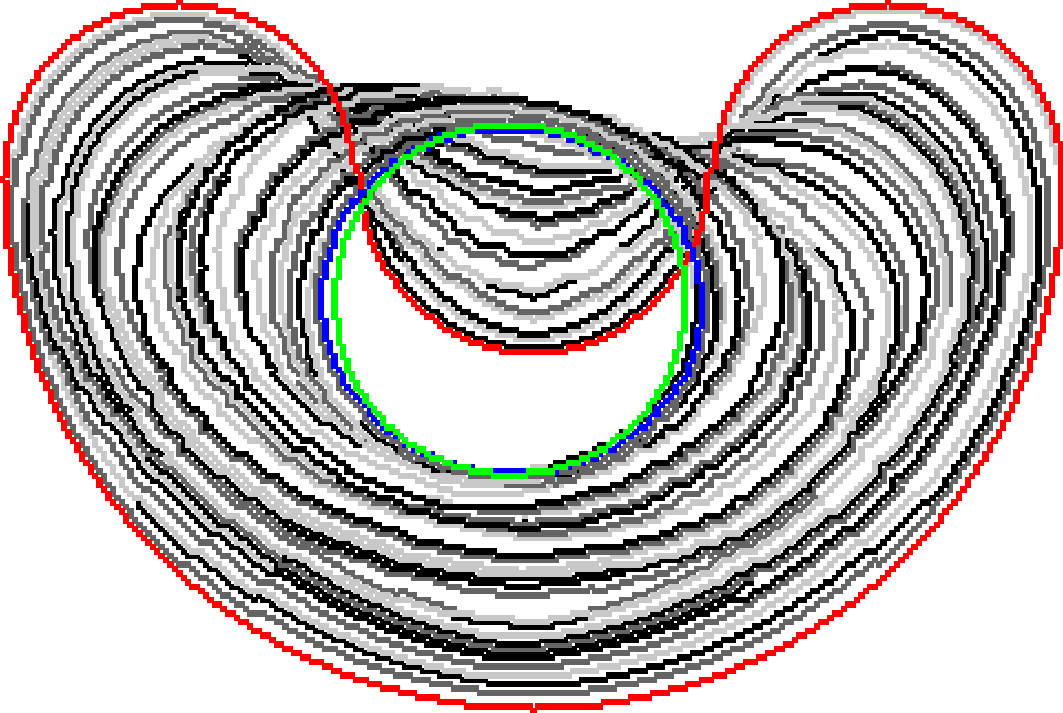
\includegraphics[scale=0.25]{figures/chapter5/flow/bean/radius_5/ii/elastica/len_pen_0.01000/jonctions_1/best/gs_0.25000/summary.pdf}\\[2em]			

	
	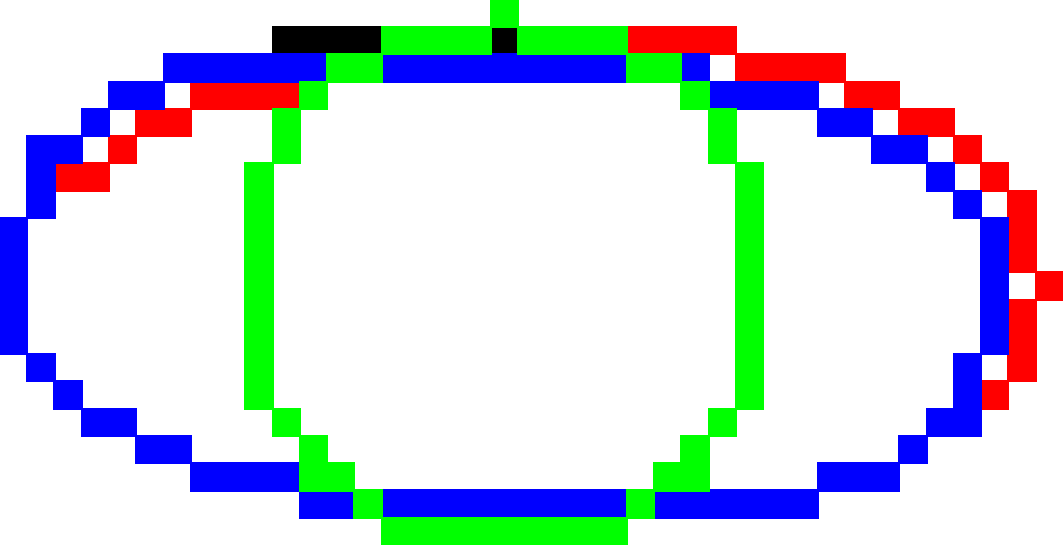
\includegraphics[scale=0.25]{figures/chapter5/flow/ellipse/radius_5/ii/elastica/len_pen_0.01000/jonctions_1/best/gs_1.00000/summary.pdf} &

	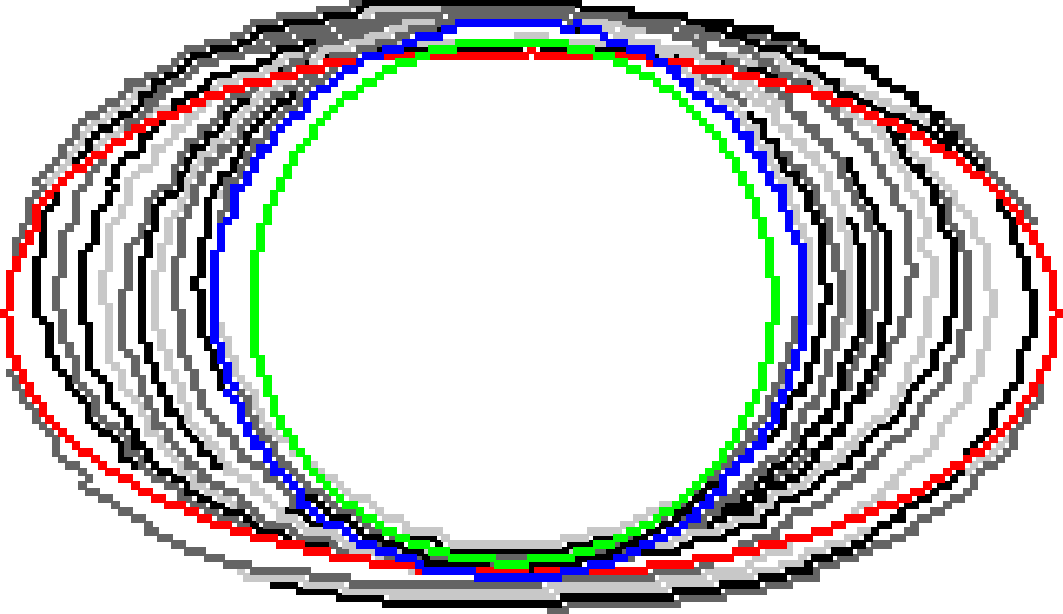
\includegraphics[scale=0.25]{figures/chapter5/flow/ellipse/radius_5/ii/elastica/len_pen_0.01000/jonctions_1/best/gs_0.25000/summary.pdf} &

	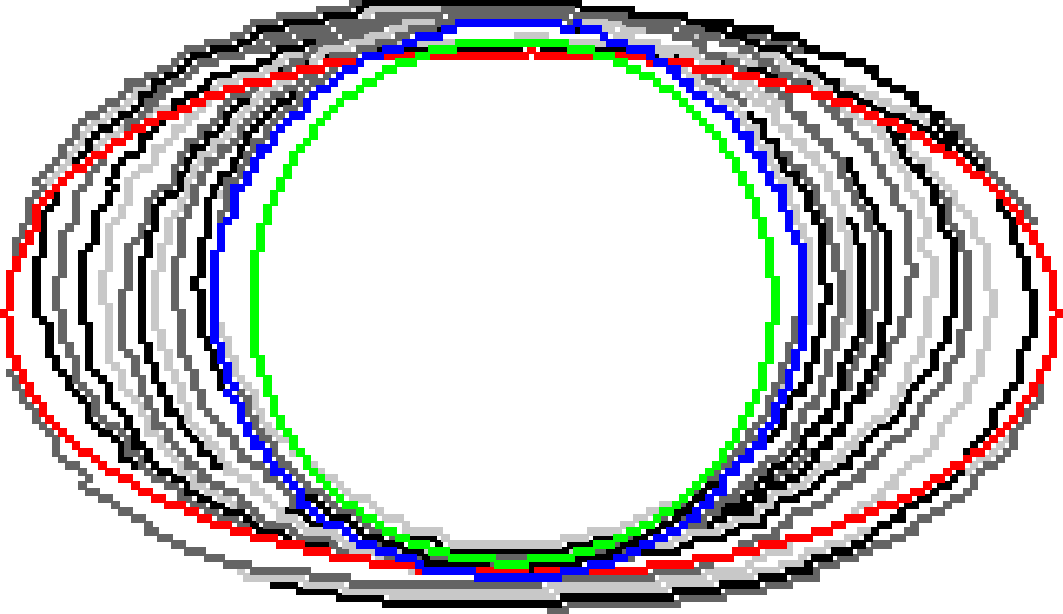
\includegraphics[scale=0.25]{figures/chapter5/flow/ellipse/radius_5/ii/elastica/len_pen_0.01000/jonctions_1/best/gs_0.25000/summary.pdf}				
\end{tabular}
		\caption{Local combinatorial optimization process results for several shapes with $\alpha=0.01,\beta=1$. The initial contour is colored in red; the final contour is colored in blue; and the optimal contour is colored in green.}	
		\label{fig:local-comb-ii5-results}
\end{figure}

\begin{figure}
\center
\begin{tabular}{ccc}
$h=1.0$ & $h=0.5$ & $h=0.25$\\[2em]
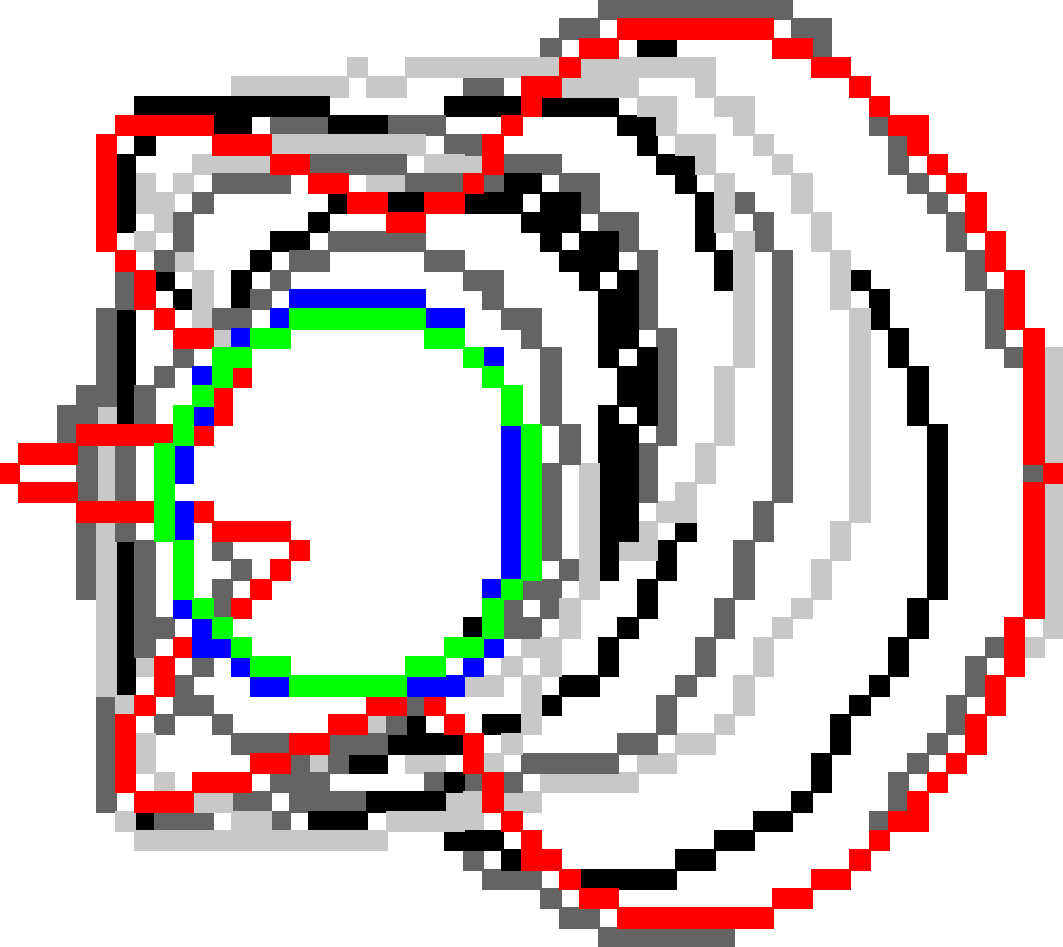
\includegraphics[scale=0.25]{figures/chapter5/flow/flower/radius_3/mdca/elastica/len_pen_0.01000/jonctions_1/best/gs_1.00000/summary.pdf} &
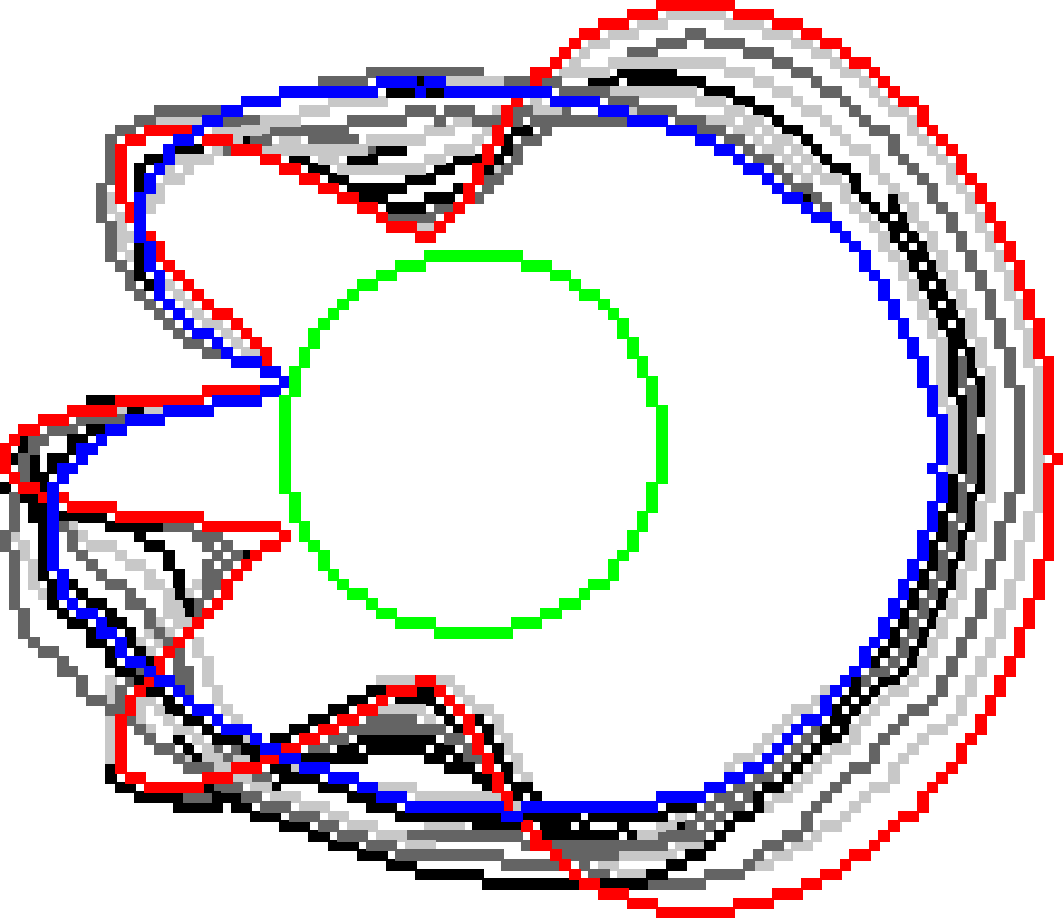
\includegraphics[scale=0.25]{figures/chapter5/flow/flower/radius_3/mdca/elastica/len_pen_0.01000/jonctions_1/best/gs_0.50000/summary.pdf} &
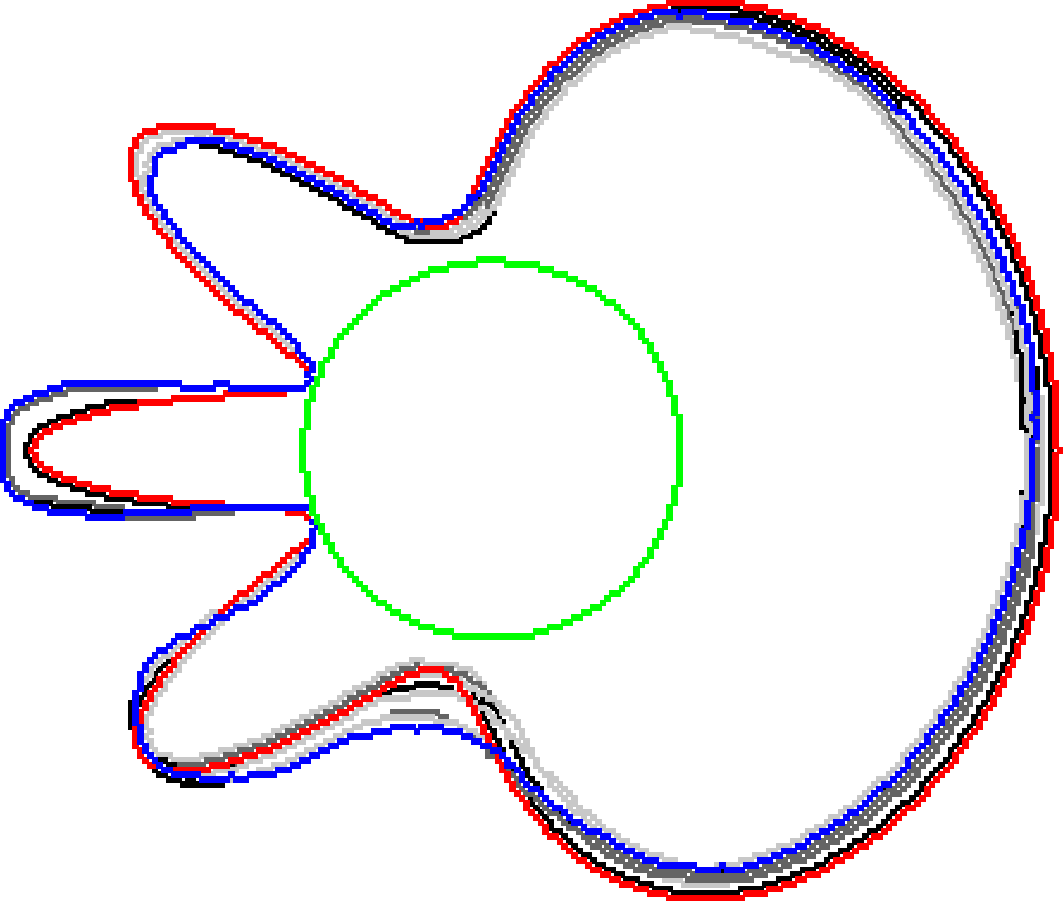
\includegraphics[scale=0.25]{figures/chapter5/flow/flower/radius_3/mdca/elastica/len_pen_0.01000/jonctions_1/best/gs_0.25000/summary.pdf}\\[2em]
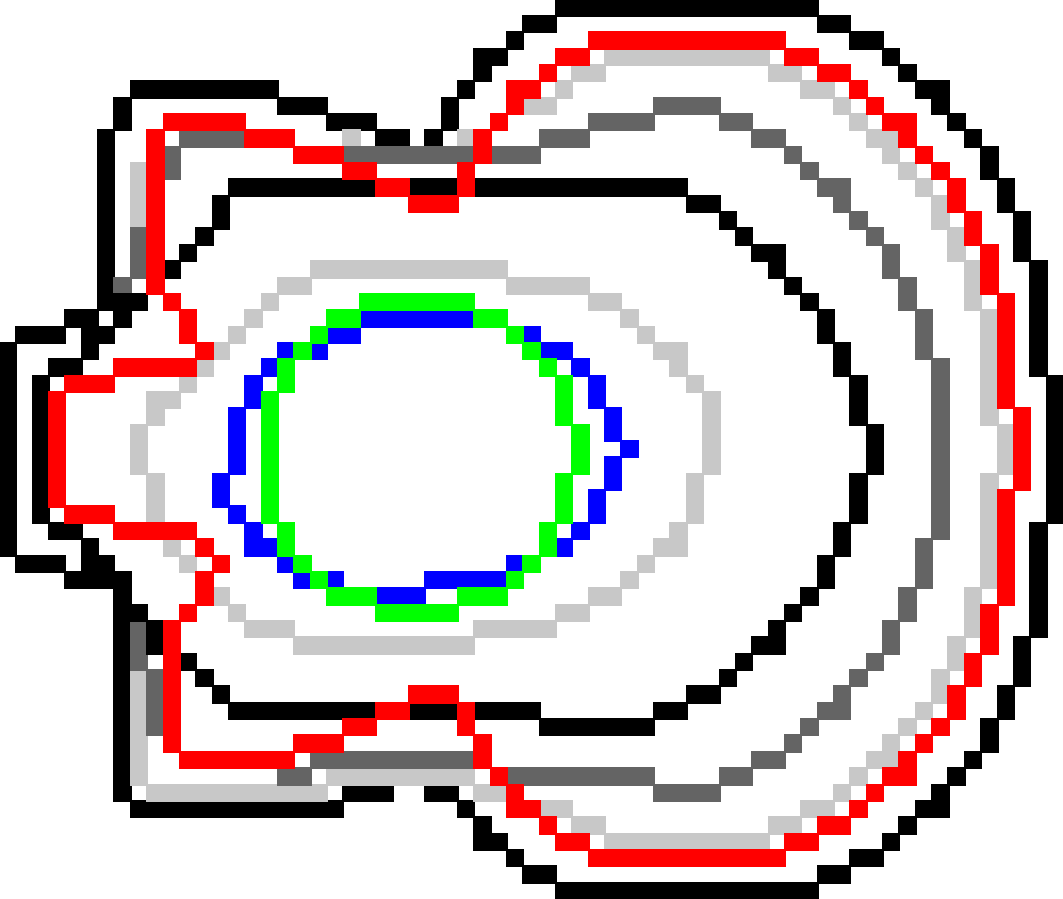
\includegraphics[scale=0.25]{figures/chapter5/mdca-larger-neighborhood/flower/0.01/1.0/summary.pdf} &
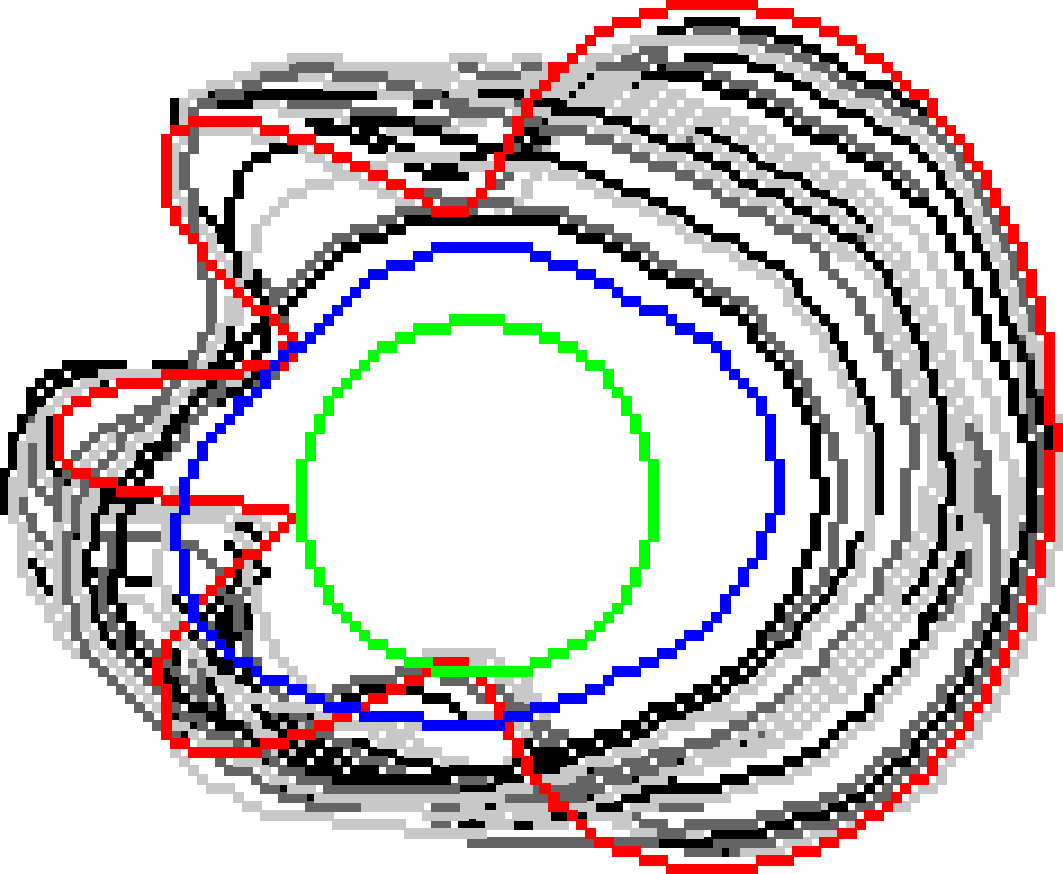
\includegraphics[scale=0.25]{figures/chapter5/mdca-larger-neighborhood/flower/0.01/0.5/summary.pdf} &
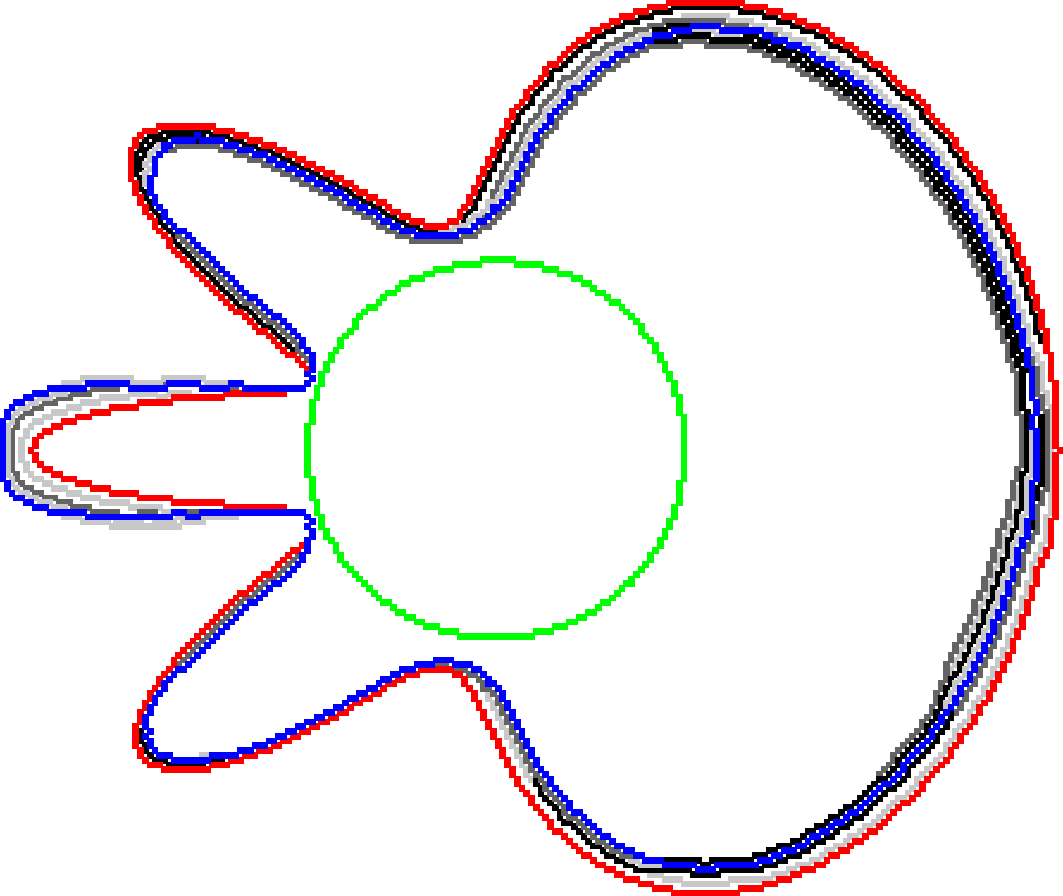
\includegraphics[scale=0.25]{figures/chapter5/mdca-larger-neighborhood/flower/0.01/0.25/summary.pdf}
\end{tabular}
\caption{In the top row, the MDCA evolution for the neighborhood as presented in algorithm \ref{alg:local-search}. In the bottom row, the flow using the extended neighborhood. The extended neighborhood additionaly includes the dilation and erosion of the initial shape by a square of side $1$.}
\label{fig:mdca-larger-neighborhood}
\end{figure}


The algorithm is suitable for any type of digital estimator. To estimate length we use MDSS and to estimate curvature we execute experiments with the MDCA and II-$r$ estimators ($r$ denoting the radius of the estimation ball). 


\subsection{Free Digital Elastica}
In the free digital elastica energy we optimize energy \ref{eq:digital-elastica} without any constraint. We observe that for $\alpha=0, \beta >0$ the Elastica becomes the integration of the squared curvature integration along the shape contour which has the ball of infinite radius as its minimizer. For $\alpha > 0, \beta=0$, minimize Elastica becomes minimize perimeter (curvature flow). It is easy to see that for $\alpha, \beta > 0$, the optimal shape for the Elastica is a disk of radius $r$. We can easily find the value of $r$.

\begin{align*}
	\frac{d}{dr}\big( \int_{\partial B(r)}{ (\alpha + \beta \kappa ^2) ds} \big ) &= 0\\
	\frac{d}{dr}\big( \alpha 2\pi r + \beta \pi/r \big) &= 0\\
	r &= \alpha^{-1/2}.
\end{align*}  

Therefore, the optimal shape for the free digital elastica is a digital disk of finite radius $\alpha^{-1/2}$.


In figure \ref{fig:local-comb-ii5-results} we present several flows derived by algorithm \ref{alg:local-search} for parameters $\alpha=0.01, \beta=1$. We observe that both II-$5$ and II-$10$ evolve the shapes to disks of radius close to the optimal value of $10$ (see figure \ref{fig:local-comb-estimators-plots-lp001}). The II-$3$ estimator stops prematurely at a local optima due its limited sensibility compared to II-$5$ or II-$10$, while MDCA encounters some difficults to evolve in a high resolution setting and it also stops at some local optima. In fact, the MDCA estimator, although with higher convergence speed, is more sensitive to noise than II, as illustrated in figure \ref{fig:mdca-sensitivity}. Nonetheless, the results can be improved by using a larger neighborhood, as illustrates figures \ref{fig:mdca-larger-neighborhood}.



We've executed the same experiments for different parameters $\alpha$ to confirm the effectiveness of our approach. We observe that the plots for $\alpha=0.001$ in figure \ref{fig:local-comb-estimators-plots-lp0001} follows a pattern similar to those in figure \ref{fig:local-comb-estimators-plots-lp001} for $\alpha=0.01$. In particular, the remarks for the II-$3$ and MDCA estimator are the same. Further, we point out that II-$5$ values are slightly farther from the optima for $\alpha=0.001$. The reason being that the shapes evolve to a ball of higher radius compared to the case $\alpha=0.01$. At some point of the evolution for $\alpha=0.001$, the sensibility of II-$5$ is not sufficient to escape from local optima. We remark that the adoption of an automatic selection of the estimation ball radius may attenuate this problem.


\begin{figure}[]
\begin{minipage}[b]{0.6\textwidth}
\center
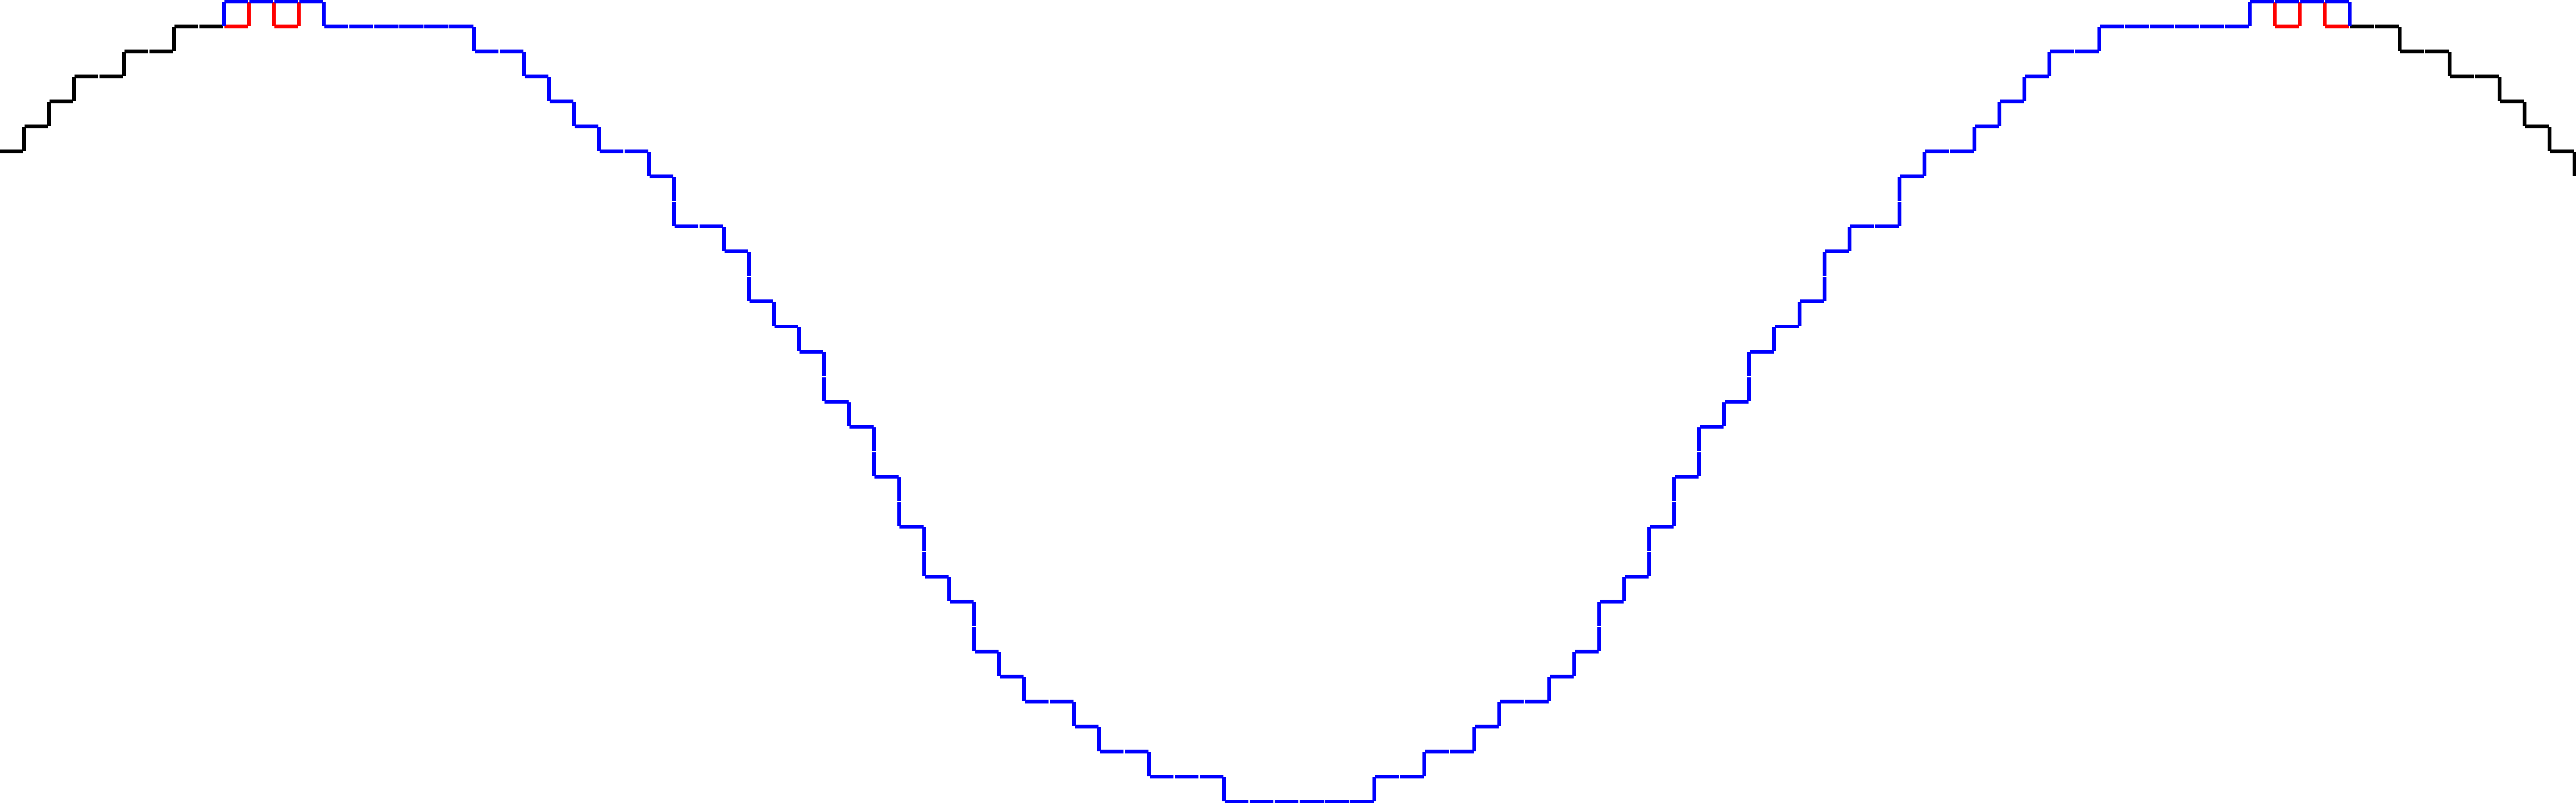
\includegraphics[scale=0.15]{figures/chapter5/mdca-sensitivity/closer-picture.pdf}
\end{minipage}%
\begin{minipage}[b]{0.4\textwidth}
\center
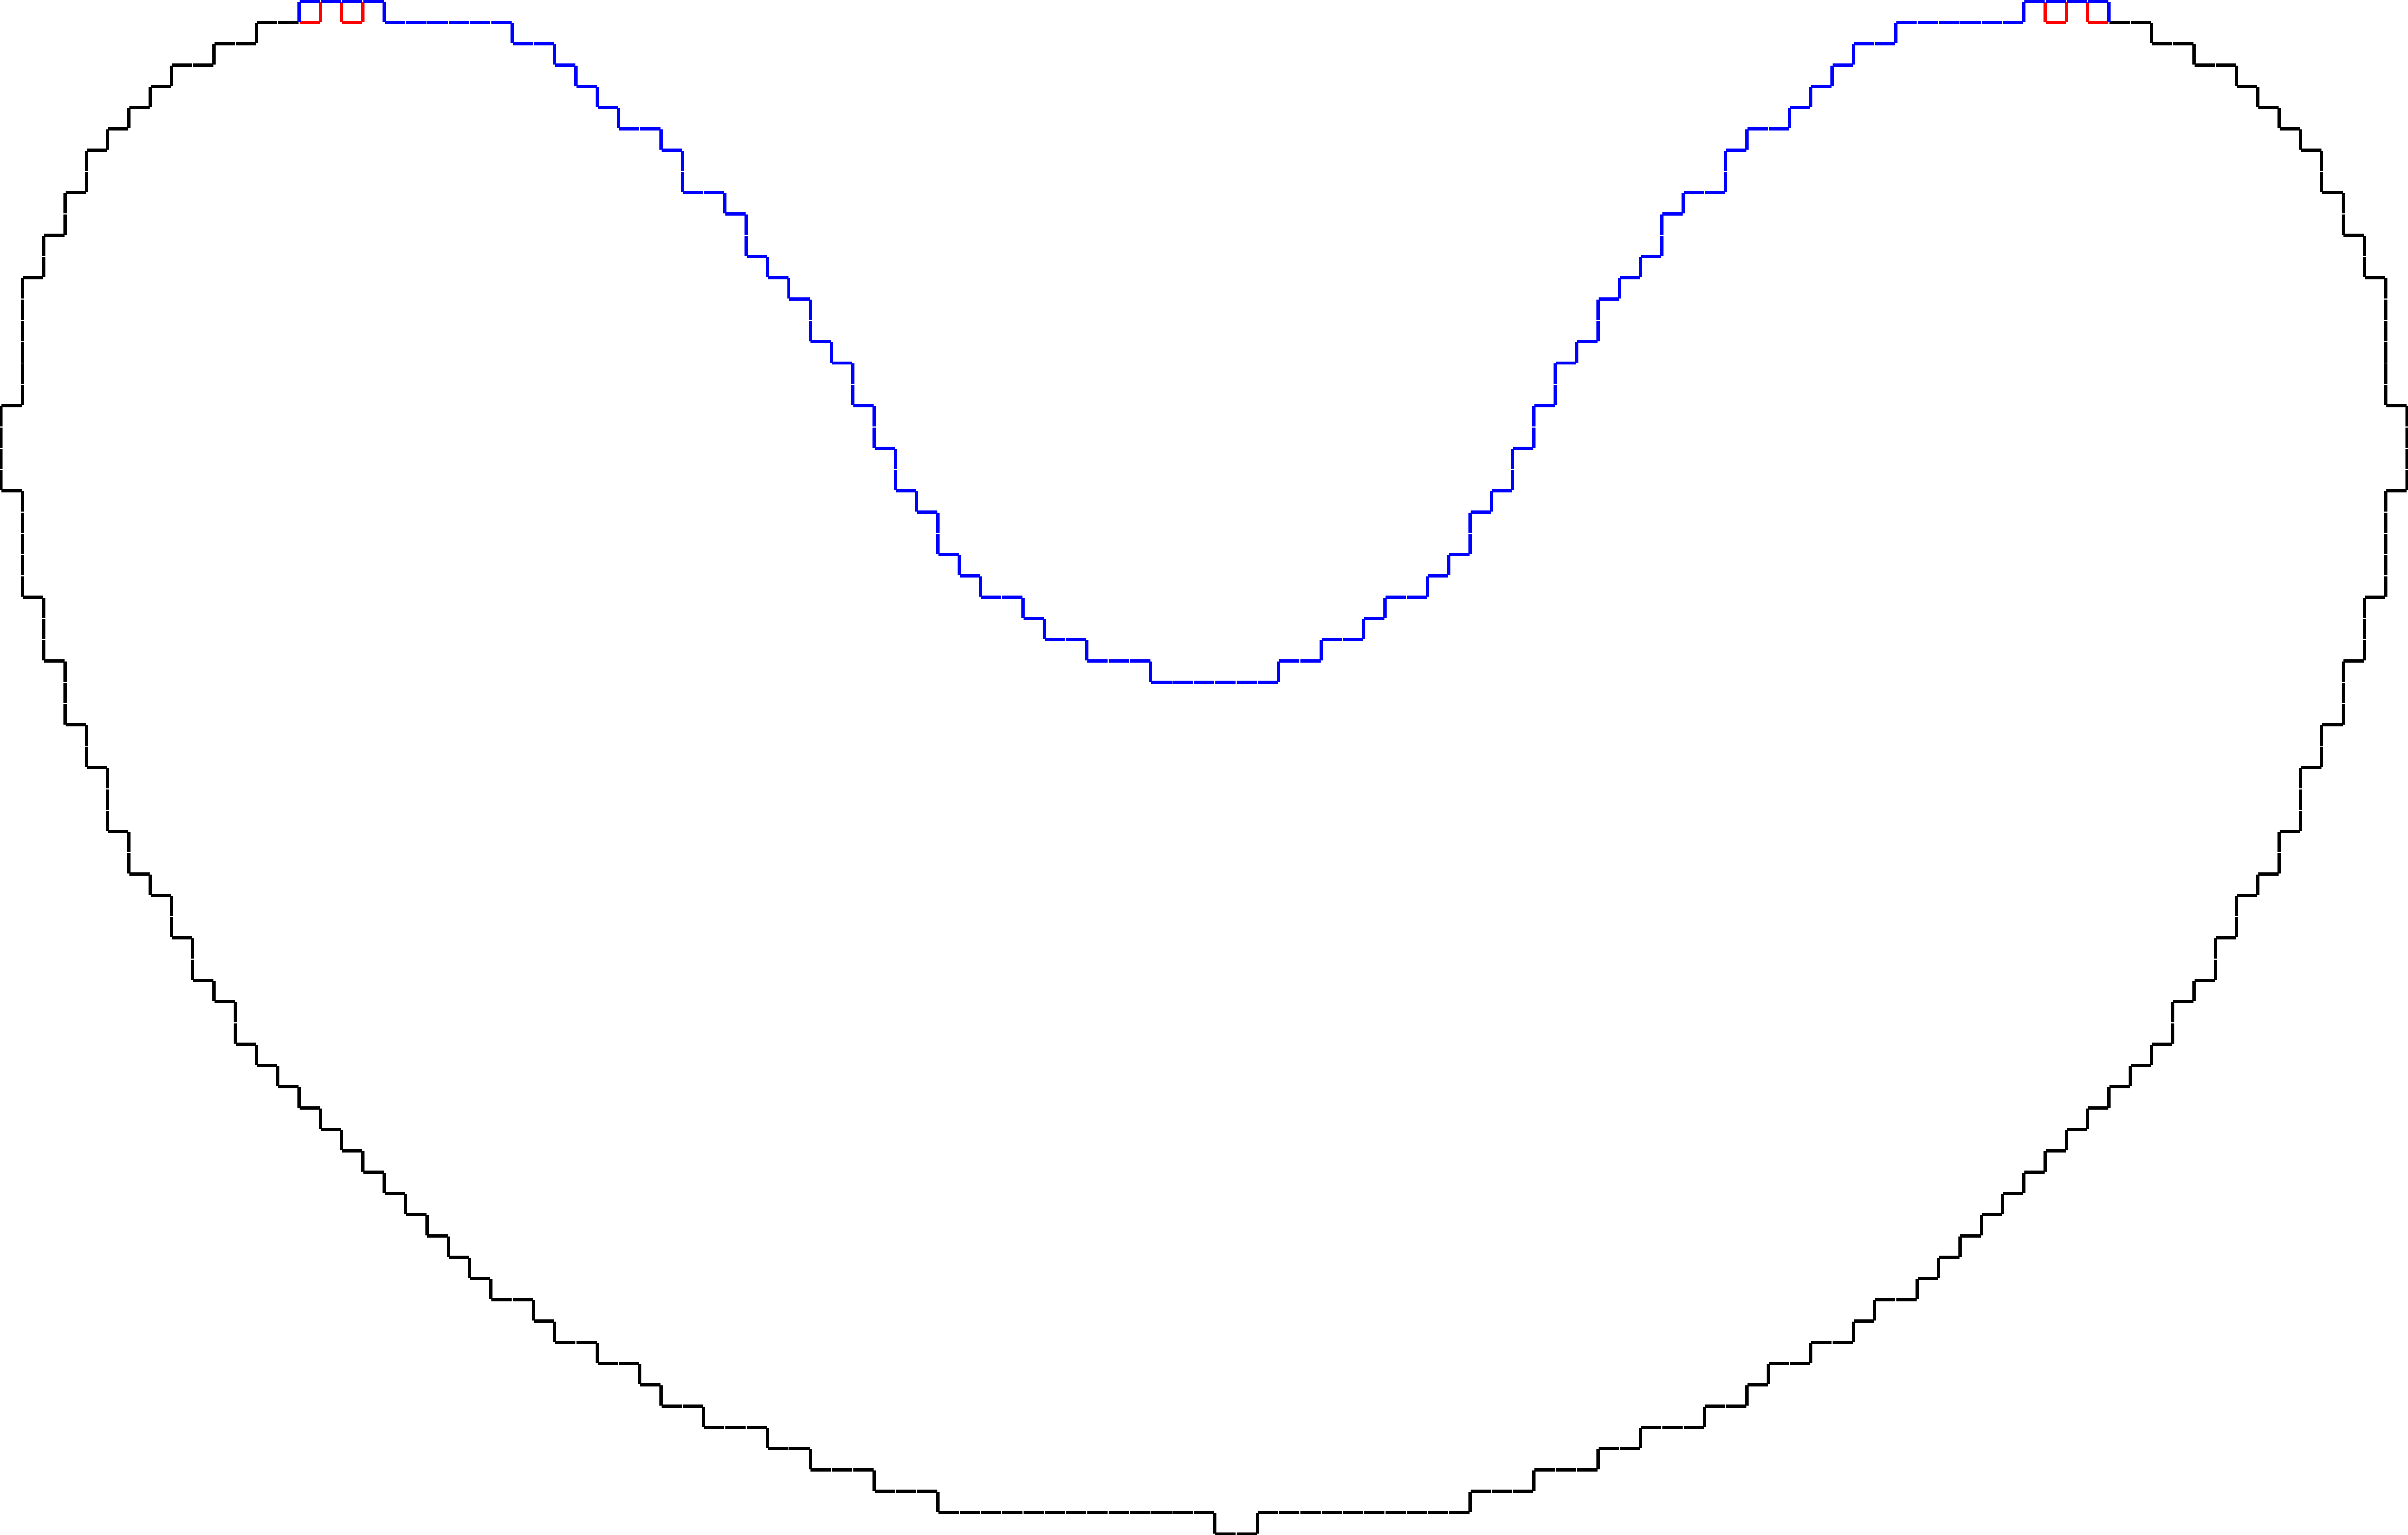
\includegraphics[scale=0.025]{figures/chapter5/mdca-sensitivity/big-picture.pdf}\\\vspace{2em}
\captionsetup{type=table}
\begin{tabular}{r|c|c}
& II-$5$ & MDCA \\
\hline
Red  & 5.54 & 3.93\\
Blue & 5.55 & 3.84\\
\hline
$| \Delta E / \Delta S |$ & 70 & 1400
\end{tabular}
\end{minipage}
\caption{A slight variation in the shape boundary (in this example, a $0.07\%$ change or $4$ pixels over $5310$) inflicts a considerably higher change in the energy value when using MDCA than when using II. }
\label{fig:mdca-sensitivity}
\end{figure}

\subsection{Constrained Digital Elastica}

An important advantage of algorithm \ref{alg:local-search} is that constraints can be imposed with minimum effort. We present results for two types of constraints. In the first type, we force some pixels to be part of the final solution and in the second we impose orientations at the endpoints of a curve. In figure \ref{fig:constrained-elastica} we compare the flows for different values of $\alpha$.


\begin{figure}
\center
\begin{tabular}{ccc}
$\alpha=0.1$ & $\alpha=0.01$ & $\alpha=0.001$\\[2em]
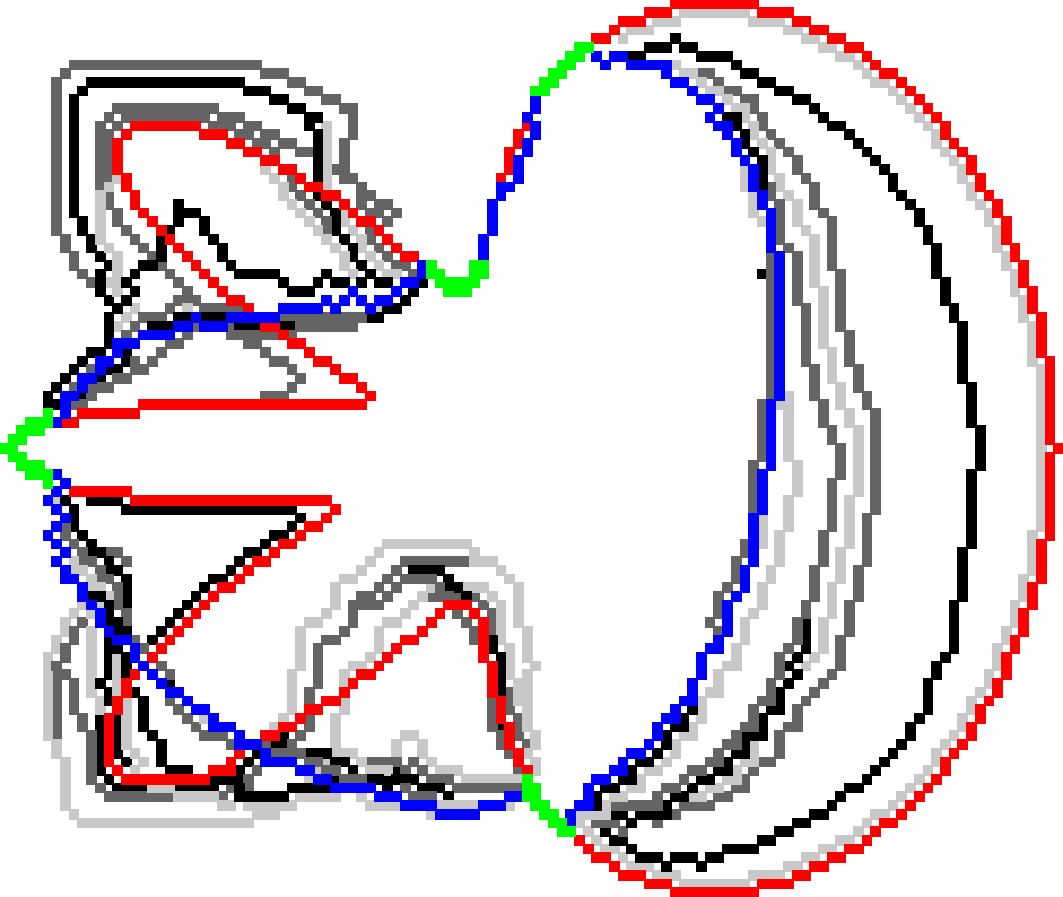
\includegraphics[scale=0.25]{figures/chapter5/fixed-pixels/elastica/len_pen_0.1/flower-1/summary.pdf} &
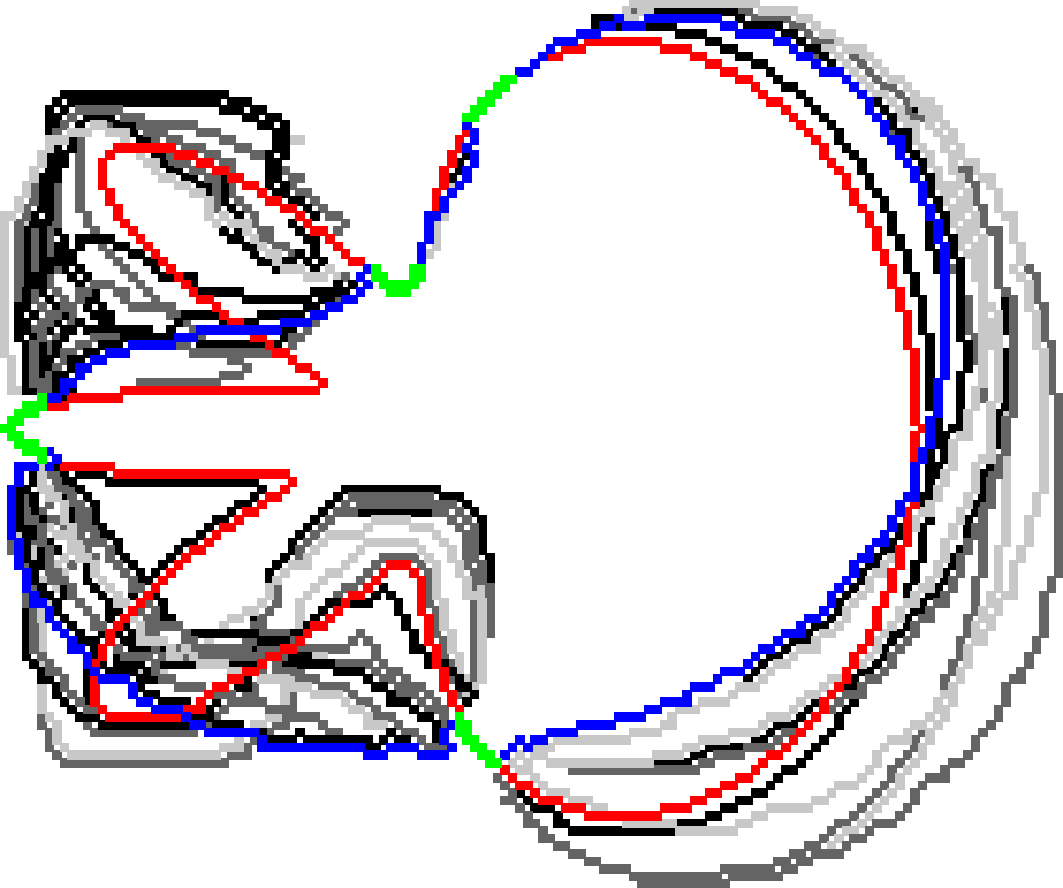
\includegraphics[scale=0.25]{figures/chapter5/fixed-pixels/elastica/len_pen_0.01/flower-1/summary.pdf} &
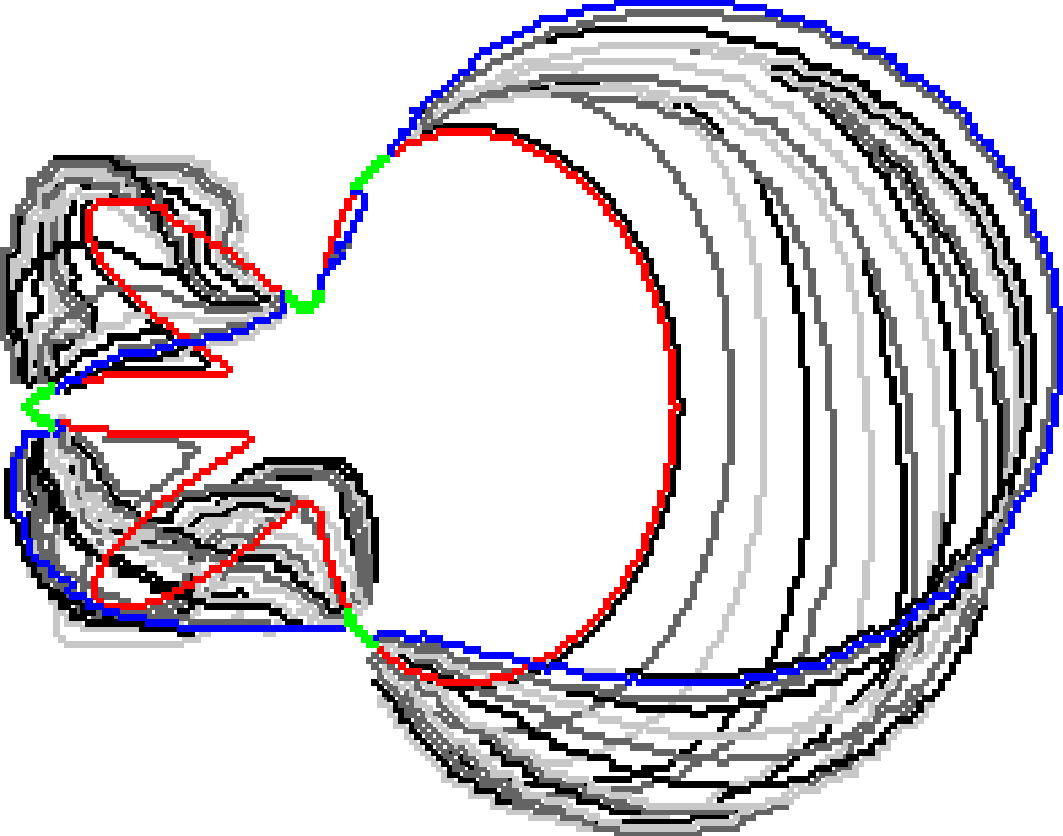
\includegraphics[scale=0.25]{figures/chapter5/fixed-pixels/elastica/len_pen_0.001/flower-1/summary.pdf}\\[2em]
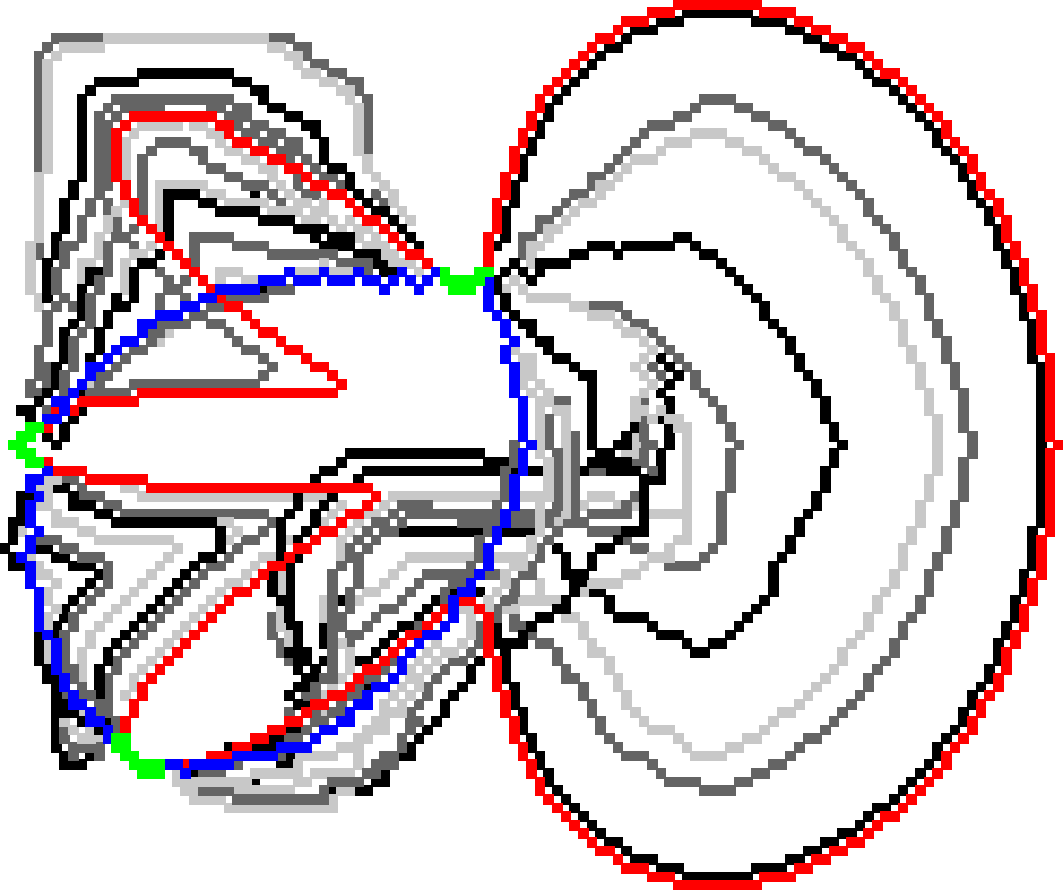
\includegraphics[scale=0.25]{figures/chapter5/fixed-pixels/elastica/len_pen_0.1/flower-2/summary.pdf} &
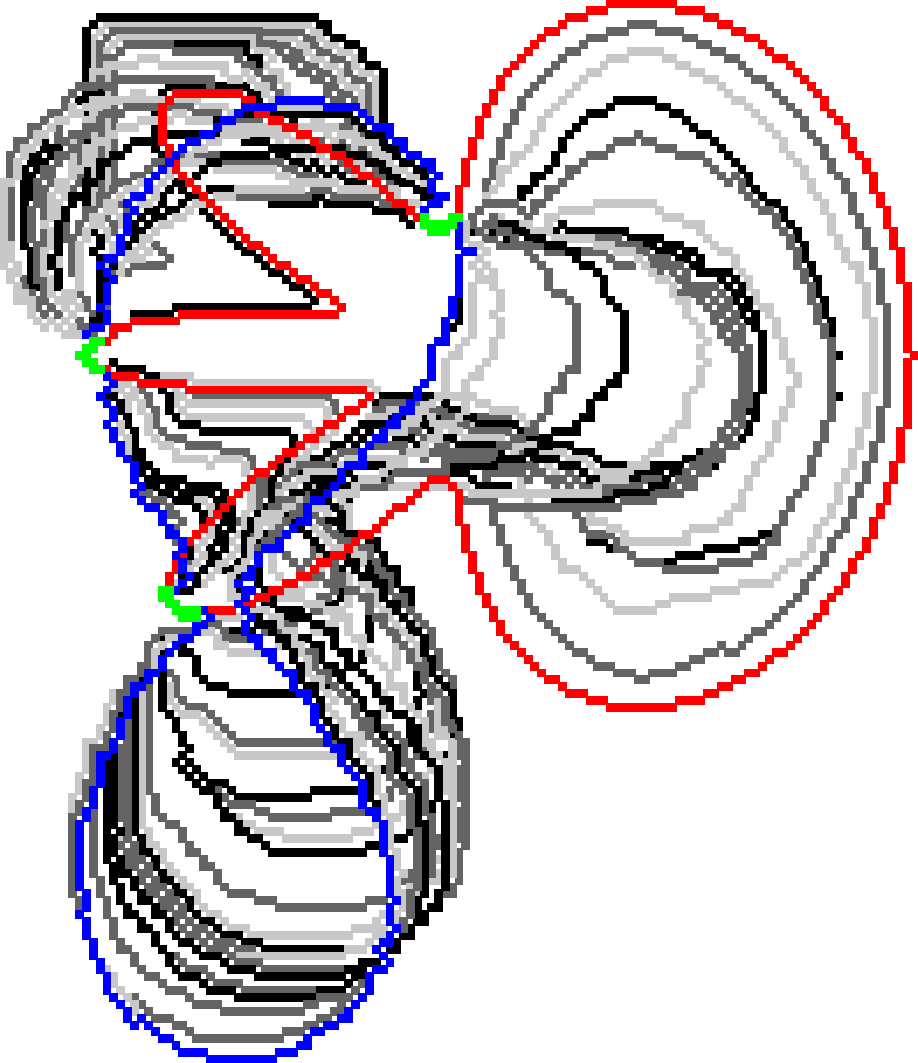
\includegraphics[scale=0.25]{figures/chapter5/fixed-pixels/elastica/len_pen_0.01/flower-2/summary.pdf} &
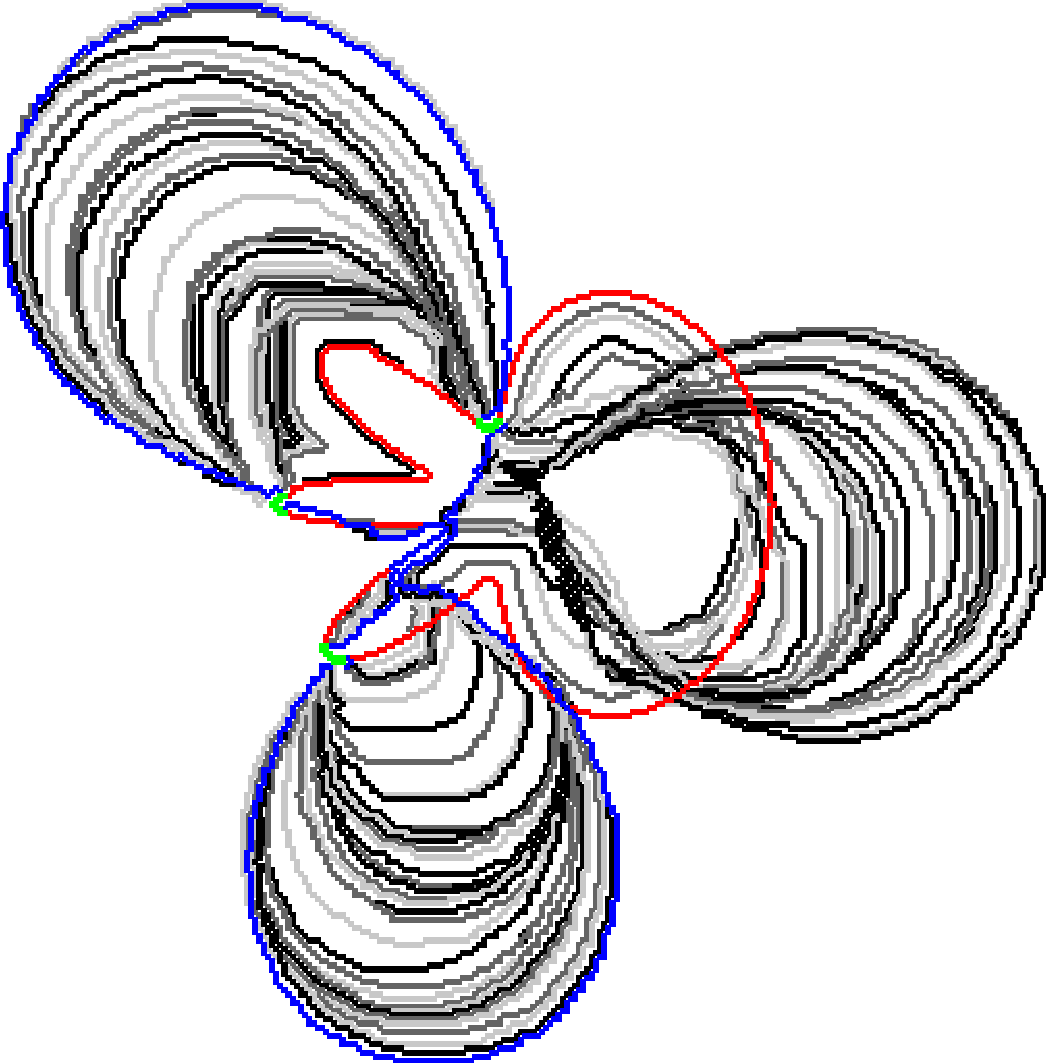
\includegraphics[scale=0.25]{figures/chapter5/fixed-pixels/elastica/len_pen_0.001/flower-2/summary.pdf}\\[2em]
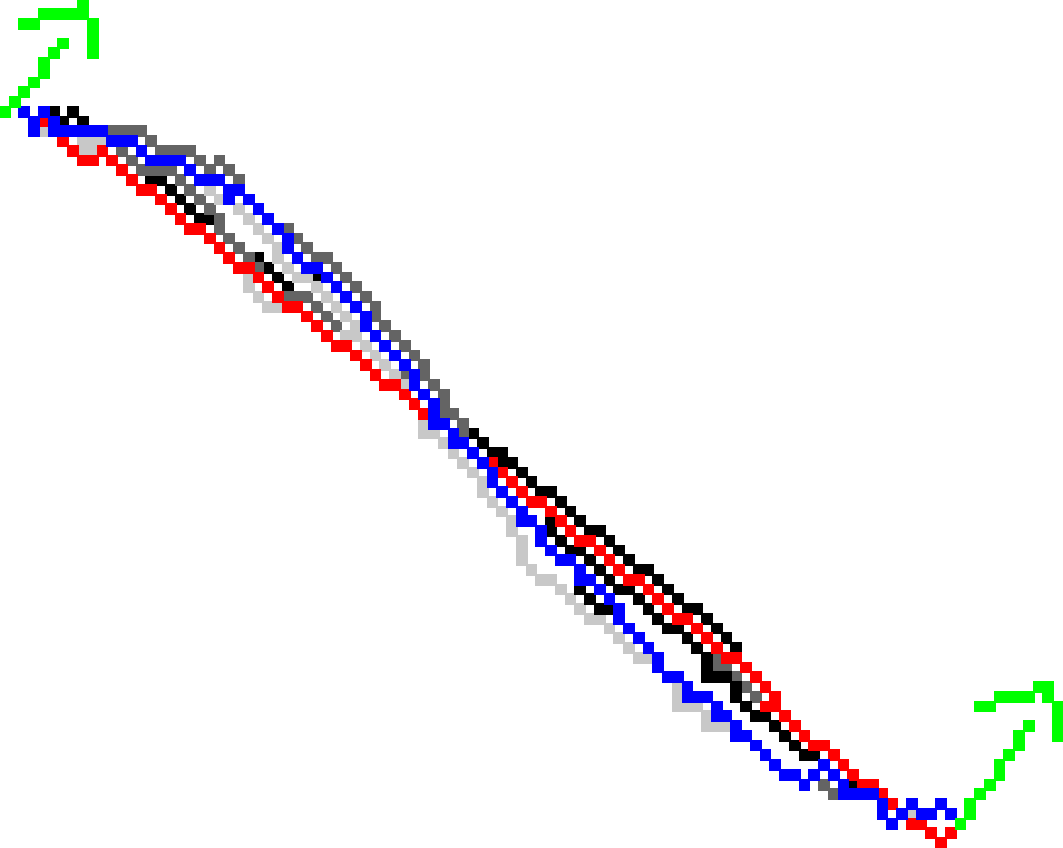
\includegraphics[scale=0.25]{figures/chapter5/fixed-orientations/elastica/len_pen_0.1/curve-2/summary.pdf} &
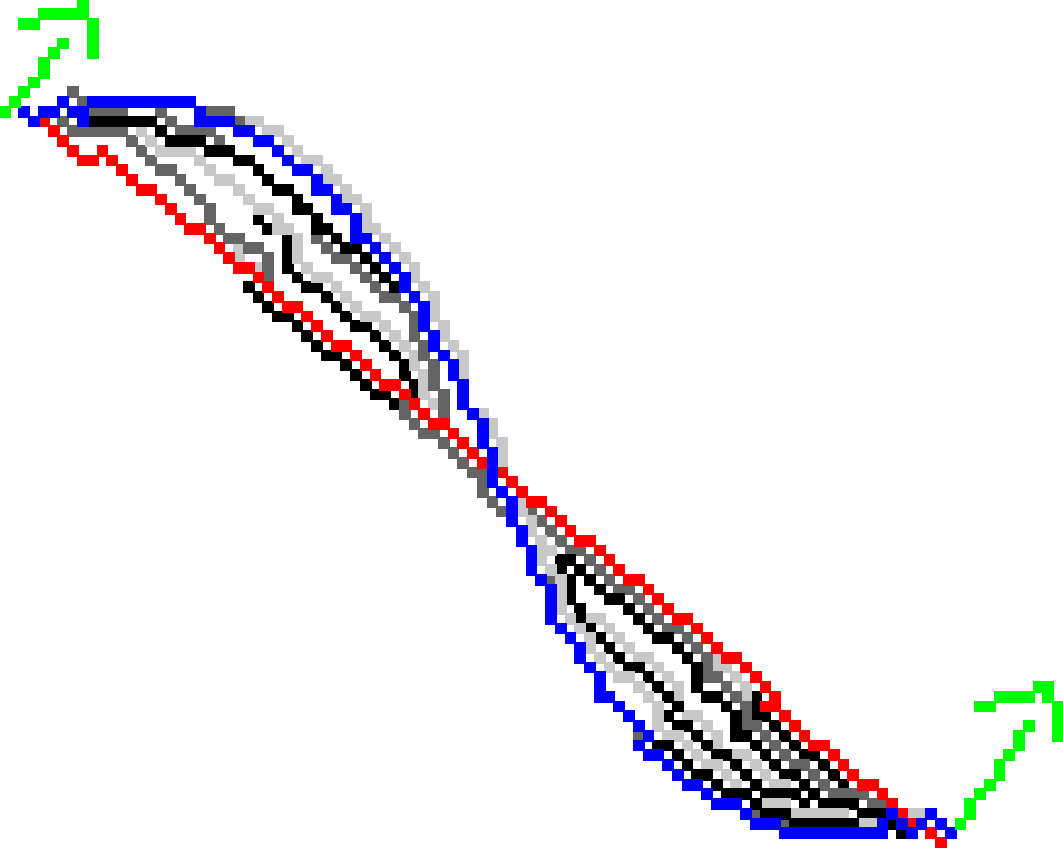
\includegraphics[scale=0.25]{figures/chapter5/fixed-orientations/elastica/len_pen_0.01/curve-2/summary.pdf} &
\includegraphics[scale=0.25]{figures/chapter5/fixed-orientations/elastica/len_pen_0.001/curve-2/summary.pdf}\\[2em]
\includegraphics[scale=0.25]{figures/chapter5/fixed-orientations/elastica/len_pen_0.1/curve-3/summary.pdf} &
\includegraphics[scale=0.25]{figures/chapter5/fixed-orientations/elastica/len_pen_0.01/curve-3/summary.pdf} &
\includegraphics[scale=0.25]{figures/chapter5/fixed-orientations/elastica/len_pen_0.001/curve-3/summary.pdf}
\end{tabular}
\caption{In the first and second rows, the flow obtained by forcing the green pixels to be part of the final solution; In the last two rows, the flow obtained by forcing the orientation at the endpoints of the curves.}
\label{fig:constrained-elastica}

\end{figure}

\subsection{Running time}

The running time of algorithm \ref{alg:local-search} is summarized in table \ref{tab:summary-local-comb-rtime}. All the experiments in this thesis were executed on a $32$-core $2.4Ghz$ CPU. Although its use in practical applications is
limited, we demonstrate that digital estimators are effective in their measurements and the flows evolve as expected, reaching the global optima for some shapes. We
observe that it is a complete digital approach, and we do not suffer from discretization and rounding problems, a common
issue in continuous models.  Furthermore we have checked that this approach works indifferently with Integral Invariant
curvature estimator and Maximal Digital Circular Arc curvature estimator. So the convergence of the digital curvature
estimator seems to be the cornerstone to get a digital curve behaving like a continuous Elastica. 

\begin{figure}[h!]
\center
\captionsetup{type=table}
\begin{tabular}{|l|c|c|c|c|c|c|}
\hline
& \multicolumn{2}{c|}{$h=1.0$} & \multicolumn{2}{c|}{$h=0.5$} & \multicolumn{2}{c|}{$h=0.25$}\\
\hline
& Pixels & Time & Pixels & Time & Pixels & Time\\
\hline
Triangle & 521 & 2s (0.05s/it)  & 2080 & 19s (0.3s/it) & 8315 & 261s (1.7s/it)\\
Square & 841 & 0.9s (0.06s/it) & 3249 & 6s (0.18s/it) & 12769 & 57s (1s/it)\\
Flower & 1641 & 6s (0.14s/it) & 6577 & 67s (0.7s/it) & 26321 & 1094s (4.7s/it)\\
Bean  & 1574 & 6s (0.1s/it) & 6278 & 76s (0.67s/it) & 25130 & 692s (3s/it)\\
Ellipse  & 626 & 1s (0.3s/it) & 2506 & 8s (0.19s/it) & 10038 & 134s (1.3s/it)\\
\hline
\end{tabular}
\caption{Running time and input size for different grid steps.}
\label{tab:summary-local-comb-rtime} 
\end{figure}





\section{Global Optimization}\label{sec:global-optmization-model}

In this section we turn to a global optimization approach. However, instead of minimizing energy \eqref{eq:digital-elastica} we are going to optimize a simplified version of it in which we don't need to compute the local length estimator.

\subsection{Simplified Digital Elastica}

The simplified digital elastica is defined as

	\begin{align}
	\hat{E}_S( D_h(X) ) = \sum_{\dot{\vec{e}} \in \partial D_h(X)}{ \alpha + \beta \hat{\kappa}_{r}^2(D_h(X),\dot{\vec{e}},h) }.
	\label{eq:simplified-digital-elastica}
	\end{align}
	

We argue that energy \eqref{eq:simplified-digital-elastica} is a reasonable approximation of \eqref{eq:digital-elastica}. Indeed, executing algorithm \ref{alg:local-search} for minimize the simplified digital elastica obtains very similar results to those for the digital elastica (see figure \ref{fig:simplified-elastica}).


\begin{figure}[]
\center
\begin{tabular}{ccc}
\includegraphics[scale=0.25]{figures/chapter5/flow/triangle/radius_5/ii/selastica/len_pen_0.01000/jonctions_1/best/gs_0.25000/summary.pdf} &
\includegraphics[scale=0.25]{figures/chapter5/flow/square/radius_5/ii/selastica/len_pen_0.01000/jonctions_1/best/gs_0.25000/summary.pdf} &
\includegraphics[scale=0.25]{figures/chapter5/flow/ellipse/radius_5/ii/selastica/len_pen_0.01000/jonctions_1/best/gs_0.25000/summary.pdf}\\[2em]
\includegraphics[scale=0.25]{figures/chapter5/flow/flower/radius_5/ii/selastica/len_pen_0.01000/jonctions_1/best/gs_0.25000/summary.pdf} &
\includegraphics[scale=0.25]{figures/chapter5/flow/bean/radius_5/ii/selastica/len_pen_0.01000/jonctions_1/best/gs_0.25000/summary.pdf} &
\includegraphics[scale=0.25]{figures/chapter5/fixed-pixels/selastica/len_pen_0.01/flower-1/summary.pdf}\\[2em]
\includegraphics[scale=0.25]{figures/chapter5/fixed-pixels/selastica/len_pen_0.01/flower-2/summary.pdf} &
\includegraphics[scale=0.25]{figures/chapter5/fixed-orientations/selastica/len_pen_0.01/curve-2/summary.pdf} &
\includegraphics[scale=0.25]{figures/chapter5/fixed-orientations/selastica/len_pen_0.01/curve-3/summary.pdf}
\end{tabular}
\caption{Experiments of section \ref{sec:local-combinatorial-scheme} for the simplified digital elastica.}
\label{fig:simplified-elastica}
\end{figure}


\subsection{Optimization Model for Simplified Elastica}

Differently from the previous section, the model described here is designed for the integral invariant estimator only. Let $D \in \frac{1}{2}\mathbb{Z}^2$ be the digitization of some shape $S \in \mathbb{R}^2$ using grid step $h$ in half-integer coordinates space. We assume that $D$ has $m$ pixels (located at integer coordinates) and $n$ linels (one and only one of its coordinates is $\frac{1}{2}$). Optimization variables are represented as vectors $x \in \mathbb{B}^{m},\, y \in \mathbb{B}^{n}$ and its $i$th coefficients denoted  $x_i,y_i$.  Further, let $A \in \mathbb{B}^{m\times n}$ the matrix defined as

\[
	A_{i,j} = \left\{ \begin{array}{ll}
		1,\; x_j \in B_{r}(y_i)\\
		0,\; \text{otherwise}.
	\end{array}\right.
\]

In other words, the column vector $A_i$ of $A$ represents the pixels that are in the interior of  the disk $B_{r}(y_i)$ of radius $r$ centered at $y_i$. 


\begin{align}
	\hat{E}(x,y) =& \sum_{y_i \in y}{ y_i \left(\; \alpha + \beta \hat{\kappa}_{r}^2(D,y_i) \; \right)}\\\nonumber
			   =& \sum_{y_i \in y}{ y_i \left(\; \alpha  + \beta \big( \frac{3}{r^3}(\frac{\pi}{r^2} - |B_r(y_i)|)\big)^2\right)}\\\nonumber
			   =& \sum_{y_i \in y}{ y_i \left(\; \alpha + \frac{9}{r^6}\beta \big(c^2 - 2cA_i^T\vec{x} + \vec{x}^TA_iA_i^T\vec{x}\big)\right)},			   
	\end{align}
	
where $c =  \pi r^2/2$. We remark that linels and pixels in the solution must be topologicaly consistent, .i.e., linels must form connected closed curves and the pixels must lie in the interior of those curves. This restriction is encoded in a set of topological constraints $T(x,y)$ detailed later. So far we have

\begin{align*}
	\min_{x \in \mathbb{B}^{|X|}, y \in \mathbb{B}^{|Y|}}{\hat{E}(x,y)}, \quad \text{subject to } T(x,y). \quad (P0)
\end{align*}

Additionaly, in real applications involving the minimization of Elastica, we have a set of constraints $R$ that plays the role of regularization. For example, we may force some of the pixels in the original shape to be part of the solution; for imaging problems, we may add a data attachment term, and so on. Finally, we can write the general optimization problem as

\begin{align*}
	\min_{x \in \mathbb{B}^{|X|}, y \in \mathbb{B}^{|Y|}}{\hat{E}(x,y)}, \quad \text{subject to } T(x,y), R(x) \quad (P1)
\end{align*}

	Formulation $P1$ is a constrained binary non-convex third order problem and likely difficult to be solved optimally. Nonetheless, we can use standard optimization techniques to acquire some intuition on the model. 	
	
\subsection{Topological constraints}

The estimation ball should be applied in the digital boundary of the shape, which oblige us to impose topological constraints in the model to avoid inconsistent solutions. In order to accomplish that, we set an arbitraty orientation for the faces and another for the edges. We choose counter-clockwise for faces; right for horizontal edges; and up for vertical edges.


For each linel $y_i$ we create variables $z_{2i},z_{2i+1}$, one for each possible orientation $y_i$ may assume. We denote this extended set as $Z$. Next, we extend the linel incidence matrix defined in appendix \ref{chapter:pixel-incidence-matrix} to hold incidence with respect to oriented edges. The new matrix $\mathbf{C} \in \mathbb{B}^{n \times m + 2n}$ is defined as

\[
	0 \leq j < m, \quad \mathbf{T}_{i,j} = \left\{ \begin{array}{ll}
	
	1,& \text{Pixel $j$ is positive incident to linel $i$}\\
	-1,& \text{Pixel $j$ is negative incident to linel $i$}\\	
	0,& \text{otherwise},
	\end{array}\right.
\]

\[
	m \leq j < m + 2n, \quad \mathbf{T}_{i,j} = \left\{ \begin{array}{ll}
	
	1,& \text{Edge $j$ is positive incident to linel $i$}\\
	-1,& \text{Edge $j$ is negative incident to linel $i$}\\	
	0,& \text{otherwise}.
	\end{array}\right.
\]

Rewriting formulation (P1)

\[
\begin{array}{ll}
& \displaystyle	\min \sum_{z_i \in Z}{ z_i \left(\; \alpha + \frac{9}{r^6}\beta \big(c^2 - 2cA_i^T\vec{x} + \vec{x}^TA_iA_i^T\vec{x}\big)\right)} \\
\text{subject to}\\
&	\mathbf{T}[ \mathbf{x}, \mathbf{z}] = 0,\\
&   R(\mathbf{x}),\\
&   \mathbf{x} \in \mathbb{B}^{m}, \mathbf{z} \in \mathbb{B}^{2n}.
\end{array}
\]


We observe that for a linel $y_i$, constraints $\mathbf{T}$ allows its both edge variables $z_{2i},z_{2i+1}$ to be evaluated to one. However, since we are minimizing a squared energy, this doesn't pose an issue.




\subsection{Linear relaxation of $P1$}

	The simplest model we can derive from (P1) consists in to relax the optimization variables to be in $\mathbb{U}$, and linearize all second and third order terms. 
	
	Let $T_i$ be a term of the summation. A term is an ordered sequence of optimization variables. For example, the term $x_2^2x_4$ is encoded as the sequence $(x_2,x_2,x_4)$. The order of term $T_i$ is the cardinality of its sequence, and it is denoted $|T_i|$. In order to linearize (P1), for each term $T_i$ of order two or higher, we create variable $z_i$ and enforce $|T_i|+1$ new constraints in the model
	
	\begin{align*}
		z_i &\leq t, \quad \forall t \in T_i \\
		z_i &\geq \sum_{t \in T_i}{t} - |T_i| + 1.		
	\end{align*}

	The final solution $x_S$ is given by a simple rounding criteria
	
\[
	x_S(i) = \left\{ \begin{array}{ll}

		 	1,& x_S(i) > 0.5\\
		 	0,& \text{otherwise}.
 	
	\end{array}\right.
\]	

	For an instance with $n$ pixels we have about $2n$ linels. After linearization, we can expect to have up to $O(n^3)$ variables, dampening our attempts to solve it globally even for low resolution images. One can also try quadratic formulations by linearizing only the third order terms. Unfortunately, the matrix of quadratic terms is not semi-definite positive, fundamental condition for efficient optimization of the model.
	


\subsection{Unconstrained version of P1}

We can use the pixel incidence matrix defined in appendix \ref{chapter:pixel-incidence-matrix} to define an unconstrained version of P1. The linel incidence vector $\mathbf{q} \in \mathbb{Z}^n$ for pixels $\mathbf{x} \in \mathbb{B}^{m}$ is 
	
	\begin{align*}
		\mathbf{q} &= \mathbf{P} \mathbf{x}
	\end{align*}

In order to supress the sign, we define diagonal matrix $\mathbf{Q} \in \mathbb{R}^{n \times n }$ as

\begin{align*}
	\mathbf{Q} = diag(\mathbf{q})diag(\mathbf{q})
\end{align*}

Let $\mathbf{B} \in \mathbb{B}^{m\times m}$ such that column vector $\mathbf{B}_j$ represents the pixels in the interior of a disk of radius $R$ centered at pixel $i$. Finally, we define the energy as

\begin{align}
	\hat{E}(\mathbf{x}) = \frac{9}{R^6}\sum_{j}^{m}{\left( \frac{\pi R^2}{2} - \boldsymbol{\mathbbm{1}}^T{\mathbf{Q}}\mathbf{B}_j \right)^2}.
	\label{eq:unconstrained-digital-elastica}
\end{align}


The resulting energy \eqref{eq:unconstrained-digital-elastica} is of order six and therefore hard to be optimized.

\section{Conclusion}
We gave a historical review of the elastica and we defined the digital elastica energy. The local combinatorial scheme defined in section \ref{sec:local-combinatorial-scheme} can evolve different shapes guided by the minimization of digital elastica energy and it eventually reaches global optima, justifying the interest for multigrid convergent estimators. Finnaly, we sketch some global optimization models using standard techniques of optimization and point out its difficulties, suggesting that a practical global optimization model is unlikely to exist. In the next chapter we explore a model that decreases the elastica energy and that can be used in practice.

